\documentclass[11pt]{article}
\usepackage{graphicx} % Required for inserting images
\usepackage{url}
\usepackage{hyperref} % Required for hyperlinks
\usepackage{xcolor} % Required for colorings
\usepackage{enumitem}
\usepackage{float}
\usepackage{listings}
\usepackage{multicol}
\usepackage{verbatim}
\usepackage{listings}
\usepackage{placeins}
\usepackage{ulem}
\usepackage{array}

\hypersetup{
    colorlinks=true,
    linkcolor=black,
    urlcolor=green
}


% All new Custom Colors
\definecolor{javascriptColor}{RGB}{240, 210, 62}
\definecolor{htmlColor}{RGB}{255, 117, 25}
\definecolor{cssColor}{RGB}{0, 106, 235}
\definecolor{nodeColor}{RGB}{95, 166, 2}
\definecolor{reactColor}{RGB}{24, 199, 242}
\definecolor{mysqlColor}{RGB}{1, 105, 130}
\definecolor{sqliteColor}{RGB}{8, 82, 77}
\definecolor{vscodeColor}{RGB}{45, 163, 247}
\definecolor{fastAPIColor}{RGB}{0, 148, 133}
\definecolor{postgresColor}{RGB}{49, 100, 140}
\definecolor{pythonColor}{RGB}{255, 170, 51}

\lstdefinestyle{codestyle}{
    backgroundcolor=\color{gray!10},  % Set background color
    basicstyle=\ttfamily\small,       % Set font style and size
    numbers=left,                      % Show line numbers
    numberstyle=\tiny,                 % Set style for line numbers
    numbersep=5pt,                     % Set distance between line numbers and code
    breaklines=true,                   % Enable line breaking
    frame=single,                      % Add a frame around code
    framesep=5pt,                      % Set padding inside frame
    rulecolor=\color{black!70},        % Set color of frame
    captionpos=b,                      % Position of caption (b = below)
}

% All New Custom Commands
\newcommand{\projectTitle}{\textbf{TestCraft}} % Find a nice Project Title Please
\newcommand{\documentationURL}{https://github.com/saged-sama/TestCraft/}
\newcommand{\JavaScript}{\href{https://www.javascript.com/}{\textbf{\colorbox{javascriptColor}{\textcolor{black}{\textit{JavaScript}}}}}}
\newcommand{\HTML}{\href{https://html.com/}{\textbf{\textcolor{htmlColor}{\textit{HTML}}}}}
\newcommand{\CSS}{\href{https://www.w3schools.com/css/}{\textbf{\textcolor{cssColor}{\textit{CSS}}}}}
\newcommand{\NodeJS}{\href{https://nodejs.org/en}{\textit{\textbf{\textcolor{black}{N}\textcolor{nodeColor}{o}\textcolor{black}{de}\textcolor{nodeColor}{JS}}}}}
\newcommand{\ReactJS}{\href{https://react.dev/}{\textbf{\textcolor{reactColor}{\textit{ReactJS}}}}}
\newcommand{\ExpressJS}{\href{https://expressjs.com/}{\textit{\textbf{\textcolor{black}{Express}\colorbox{javascriptColor}{\textcolor{black}{JS}}}}}}
\newcommand{\MySQL}{\href{https://www.mysql.com/}{\textbf{\textcolor{mysqlColor}{\textit{MySQL}}}}}
\newcommand{\SQLite}{\href{https://www.sqlite.org/index.html}{\textbf{\textcolor{sqliteColor}{\textit{SQLite}}}}}
\newcommand{\squarebullet}{\textcolor{black}{\rule{0.26em}{0.26em}}}
\newcommand{\FastAPI}{\href{https://fastapi.tiangolo.com/}{\textbf{{\textcolor{fastAPIColor}{\textit{FastAPI}}}}}}
\newcommand{\PostgreSQL}{\href{https://www.postgresql.org/}{\textbf{{\textcolor{postgresColor}{\textit{PostgreSQL}}}}}}
\newcommand{\Python}{\href{https://www.python.org/}{\textbf{{\textcolor{pythonColor}{\textit{Python}}}}}}

% Bullet Points Setup
\newlist{customItemize}{itemize}{4}
\setlist[customItemize,1]{label=\textbullet}
\setlist[customItemize,2]{label=\textopenbullet}
\setlist[customItemize,3]{label=\squarebullet}
\setlist[customItemize,4]{label=\textasteriskcentered}

\begin{document}
\begin{titlepage}
    \begin{center}
        
\includegraphics[scale=0.10]{du.png}\par
        \begin{Huge}
            \textsc{University of Dhaka}\par
        \end{Huge}
        \begin{Large}
            Department of Computer Science and Engineering\par
            \vspace{0.5cm}
            CSE-4113 : Internet Programming Lab \\[12pt]
            Project Title: Website for CSEDU \\[12pt]
            \textbf{Requirement Analysis Document}
        \end{Large}
    \end{center}
    \vfill
    \hfill \textbf{Submission Date:} \today
    \newpage
    \begin{center}
        \begin{Large}
            \textbf{Submitted to:\\[12pt]}
            Dr. Mamun Or Rashid\\
            Redwan Ahmed Rizvee\\
            Md. Tanvir Alam\\
        \end{Large}
    \end{center}

    \vspace{5cm}

    \begin{center}   
        \begin{Large}
            \textbf{Submitted by:\\[12pt]}
            Meherun Farzana (Roll - 05) \\
            Sarower Jahan Rafin (Roll - 09) \\
            Md. Mahmudul Hasan (Roll - 10) \\
            Md. Emon Khan (Roll - 30) \\
            Diptajoy Mistry (Roll - 34) \\
            Md. Rasel Hossen (Roll - 39) \\
            Md. Mushiur Rahman (Roll - 58) \\
            Mahmudul Hasan (Roll - 60) \\
            Sabrina Hossain (Roll - 61) \\
        \end{Large}
    \end{center}

\end{titlepage}
\newpage

% Do not Touch!! Table of Contents Go Here...
\tableofcontents
\newpage

\section{Introduction}
The \textit{Department of Computer Science and Engineering} (CSE) at the \textit{University of Dhaka} is a leading academic institution in Bangladesh. It offers a wide range of programs and resources for students, faculty, and staff. To support its academic and administrative activities, there is a need for a centralized, interactive, and efficient application platform. This platform will serve as a digital hub for accessing academic resources, managing administrative tasks, and enabling communication among participants. The goal of this project is to design and develop a scalable and user-friendly system that fulfills the needs of the department, using modern tools and technologies.

\subsection{Purpose of the System}
The purpose of this system is to create a digital platform that improves the academic and administrative experience for students, faculty, and staff within the \textit{Department of Computer Science and Engineering}. The system will provide academic resources, administrative processes, and better communication and collaboration.

\subsection{Scope of the System}
The scope of this project includes the following key features:

\begin{itemize}
    \item \textbf{User Management:} Support for multiple user roles (students, faculty, admin) with role-based access control.
    \item \textbf{Academic Resources:} A repository for course materials, syllabi, lecture notes, and research papers.
    \item \textbf{Announcements:} Updates on important events, deadlines, and announcements.
    \item \textbf{Event Management:} Scheduling and management of departmental events, seminars, workshops, and meetings.
    \item \textbf{Interactive Interface:} A modern, responsive, and user-friendly interface accessible on both desktop and mobile devices.
    \item \textbf{Database Integration:} Secure storage and retrieval of data using a relational database system.
\end{itemize}

\subsection{Objective and Success Criteria of the System}
The main objectives of this project are:

\begin{itemize}
    \item \textbf{Improve User Experience:} Develop an intuitive and responsive interface to ensure ease of use and accessibility for all users.
    \item \textbf{Automate Processes:} Automate administrative tasks to reduce manual effort, minimize errors, and improve efficiency.
    \item \textbf{Scalability:} Design the system to accommodate future growth in terms of users, data, and features.
    \item \textbf{Improve Communication:} Establish communication between students, faculty, and staff.
    \item \textbf{Data Security:} Implement powerful security measures to protect sensitive information to ensure data privacy.
\end{itemize}
The success criteria of the system are as follows:
\begin{itemize}
    \item \textbf{Functional Completeness:} All planned features (user management, academic resources, announcements, etc.) are fully implemented and operational.
    \item \textbf{User Satisfaction:} High usability scores and positive feedback from students, faculty, and staff.
    \item \textbf{Performance and Scalability:} Fast response times ($<2$ seconds) and ability to handle peak loads and future growth.
    \item \textbf{Reliability and Stability:} No critical failures, downtime, or data loss during normal usage.
    \item \textbf{Security and Data Protection:} Secure data storage, role-based access control, and compliance with security standards.
    \item \textbf{Adoption and Usage:} High adoption rates and active usage of key features.
    \item \textbf{Maintainability and Extensibility:} Well-documented, modular code base
    \item \textbf{Timely Delivery and Budget Compliance:} Completed within the agreed timeline and budget.
    \item \textbf{User Feedback and Impact:} Positive feedback and acknowledgment of the system's impact on improving workflows.
\end{itemize}

\subsection{Tools and Technologies}
The following tools and technologies will be used to design and develop the system:

\textbf{Frontend:}
\begin{itemize}
    \item \ReactJS: A \JavaScript\space library for building interactive and dynamic user interfaces.
    \item \HTML/\CSS: For structuring and styling the web pages.
\end{itemize}

\textbf{Backend:}
\begin{itemize}
    \item \FastAPI: A modern, fast (high-performance) web framework for building APIs with \Python.
    \item \PostgreSQL: A powerful, open-source relational database system for data storage and management.
\end{itemize}

\textbf{Other Tools:}
\begin{itemize}
    \item Git/GitHub: For version control and collaborative development.
    \item Docker: For containerization and deployment.
    \item Swagger: For API documentation, testing and debugging.
\end{itemize}


\subsection{References}

\begin{thebibliography}{99}

\bibitem{react} React Documentation. \textit{React – A JavaScript Library for Building User Interfaces}. Available at: \url{https://reactjs.org/docs/getting-started.html}.

\bibitem{fastapi} FastAPI Documentation. \textit{FastAPI – Modern, Fast (high-performance) Web Framework for Python}. Available at: \url{https://fastapi.tiangolo.com/}.

\bibitem{postgresql} PostgreSQL Documentation. \textit{PostgreSQL – The World's Most Advanced Open Source Relational Database}. Available at: \url{https://www.postgresql.org/docs/}.

\bibitem{docker} Docker Documentation. \textit{Docker – Develop, Ship, and Run Any Application, Anywhere}. Available at: \url{https://docs.docker.com/}.

\bibitem{postman} Postman Documentation. \textit{Postman – The Collaboration Platform for API Development}. Available at: \url{https://learning.postman.com/}.

\end{thebibliography}


\subsection{Overview}
The Department of Computer Science and Engineering (CSE) at the University of Dhaka requires a modern, centralized software platform to automate academic and administrative processes, provide better communication, and improve accessibility to resources. This project aims to design and develop a scalable and user-friendly software system to meet the needs of students, faculty, and staff.

The system will include features such as \textbf{user management, academic resource repositories, real-time announcements, event scheduling, and administrative task automation.} It will be built with \ReactJS \space for the frontend, \FastAPI \space for the backend, and \PostgreSQL \space for database management. The platform will offer a responsive and interactive interface accessible on both desktop and mobile devices.

The project focuses on improving user experience, ensuring data security, and enabling scalability for future growth. This system will serve as a tool for enhancing academic and administrative operations within the Department of CSE.



\section{Overall Description}
\subsection{Product Perspective}
The Department of Computer Science and Engineering at the University of Dhaka needs a modern software platform to handle academic and admin tasks, improve communication, and make resources easier to access.

The system will manage users, store academic materials, send announcements, schedule events, and automate admin work. It runs independently but can connect to university databases if needed.  

Built with \ReactJS\space (frontend), \FastAPI\space (backend), and \PostgreSQL\space (database), it’s designed for security, scalability, and future upgrades. The goal is to boost efficiency and make life easier for students, faculty, and staff.

\subsection{Product Functions}

The system will include the following major functions:

\textbf{User Management:}
\begin{itemize}
    \item Account Creation: Faculty and admin accounts can be created with verification.
    \item Password Recovery: Users can reset their passwords via email if forgotten.
\end{itemize}

\textbf{Academic Resources:}
\begin{itemize}
    \item Resource Repository: Access to course materials, syllabi, lecture notes, and research papers.
    \item Resource Upload: Faculty can upload and update academic resources.
\end{itemize}

\textbf{Announcements:}
\begin{itemize}
    \item Event Scheduling: Faculty and admins can schedule and manage departmental events, seminars, and workshops.
\end{itemize}

\subsection{User Profiles}

\textbf{Administrators:}
\begin{itemize}
    \item Oversee the entire system, manage user accounts, and access analytics.
    \item Responsible for system maintenance and updates.
\end{itemize}

\textbf{Faculty:}
\begin{itemize}
    \item Upload and manage academic resources.
    \item Schedule events, track attendance, and manage grades.
    \item Access administrative tools for course management.
\end{itemize}

\textbf{All(General) Users:}
\begin{itemize}
    \item Access academic resources, view grades, and submit forms.
    \item View different aspects, goals, achievements and opportunities within the department
\end{itemize}

\subsection{Constraints}

\textbf{Technology:}
\begin{itemize}
    \item The system is designed as a web application and is compatible with modern browsers (Chrome, Firefox, Edge, etc.).
    \item Mobile compatibility is ensured through responsive design, but native mobile apps are not part of the initial release.
\end{itemize}

\textbf{Time Constraints:}
\begin{itemize}
    \item Due to time limitations, advanced features such as AI-based recommendations or integration with external university systems may be deferred to future updates.
\end{itemize}

\textbf{Resource Constraints:}
\begin{itemize}
    \item The development team must work within the allocated budget and resources, focusing on main functionalities for the initial release.
\end{itemize}

\subsection{Assumptions and Dependencies}

\textbf{Assumptions:}
\begin{itemize}
    \item \textbf{User Familiarity:} Users (students, faculty, and staff) are assumed to have basic familiarity with web applications and online systems.
    \item \textbf{Technical Feasibility:} The chosen technology stack (\ReactJS, \FastAPI, \PostgreSQL) is assumed to be capable of supporting the required functionalities.
    \item \textbf{Adoption:} It is assumed that users will adopt the system positively and transition from existing processes to the new platform.
    \item \textbf{Security:} Users trust the system to handle their data securely, and it is assumed that the platform complies with the data protection standards.
\end{itemize}

\textbf{Dependencies:}
\begin{itemize}
    \item \textbf{Database Management System (\PostgreSQL):} The system relies on \PostgreSQL\space for secure and efficient data storage and retrieval.
    \item \textbf{Frontend and Backend Frameworks:} The functionality of the system depends on the effective integration of \ReactJS \space (frontend) and \FastAPI\space (backend).
    \item \textbf{Third-Party Services:} Integration with email services for password recovery is essential for user management.
    \item \textbf{Deployment Infrastructure:} The system depends on reliable hosting and deployment infrastructure (e.g., Docker, cloud services) for smooth operation.
\end{itemize}

\section{Proposed System}

\subsection{Functional Requirements}
\renewcommand{\arraystretch}{2}
\noindent
\begin{center}
\begin{tabular}{ | >{\bfseries}m{5em} | m{10cm} |  } 
  \hline
  ID & 3.2.1\\ 
  \hline
  Name & User and Administration \\ 
  \hline
  Description & 
  \begin{itemize}
      \item The system should allow the \textit{\textbf{Super Admin}} to create and manage teacher and admin accounts through institutional mails.
      \item Teachers can update their account information.
      \item Allow password resets for all accounts.
      \item Admins should be allowed to access, manipulate, and publish any data from the database into the website

  \end{itemize} \\
  \hline
  
  Priority & High\\
  \hline 
  Reference & \\
  \hline
\end{tabular}
\end{center}

\vspace{0.5cm}

\begin{center}
  \begin{tabular}{ | >{\bfseries}m{5em} | m{10cm} |  } 
    \hline
    ID & 3.2.2\\  
    \hline
    Name & Navbar \\  
    \hline
    Description & 
    \begin{itemize}
        \item Visualize University logo along with the department name
        \item Include quick links to pages, such as, Homepage, About, Admission, Teachers and Staff, Students Corner, Research, Academics, Events, Facilities and Alumni.
        \item Include quick links to login, logout pages
        \item Necessary quick links for admin
    \end{itemize} \\ 
    \hline
    Priority & High\\
    \hline 
    Reference & \\
    \hline
  \end{tabular}
  \end{center}

\begin{center}
\begin{tabular}{ | >{\bfseries}m{5em} | m{10cm} |  } 
  \hline
  ID & 3.2.3\\  
  \hline
  Name & Homepage \\  
  \hline
  Description & 
  \begin{itemize}
      \item Should display a welcome message.
      \item Show the department’s mission and vision.
      \item Provide announcements and news updates.
      \item Display upcoming events.
  \end{itemize} \\ 
  \hline
  Priority & High\\
  \hline 
  Reference & \\
  \hline
\end{tabular}
\end{center}

\vspace{0.5cm}


\begin{center}
\begin{tabular}{ | >{\bfseries}m{5em} | m{10cm} |  } 
  \hline
  ID & 3.2.4\\  
  \hline
  Name & About Us \\  
  \hline
  Description & 
  \begin{itemize}
      \item Provide an overview of the department.
      \item Include a message from the Head of the Department.
      \item Showcase department history and achievements.
      \item Show contact information and location on a map.
  \end{itemize} \\ 
  \hline
  Priority & Medium\\
  \hline 
  Reference & \\
  \hline
\end{tabular}
\end{center}

\vspace{0.5cm}


\begin{center}
\begin{tabular}{ | >{\bfseries}m{5em} | m{10cm} |  } 
  \hline
  ID & 3.2.5\\  
  \hline
  Name & Academics \\  
  \hline
  Description & 
  \begin{itemize}
      \item Provide information about undergraduate, postgraduate, and PhD programs.
      \item Display course structures, syllabi, and credit details.
      \item Include class schedules and timetables.
      \item Provide an academic calendar with important dates.
  \end{itemize} \\ 
  \hline
  Priority & High\\
  \hline 
  Reference & \\
  \hline
\end{tabular}
\end{center}

\vspace{0.5cm}

\begin{center}
  \begin{tabular}{ | >{\bfseries}m{5em} | m{10cm} |  } 
    \hline
    ID & 3.2.5\\  
    \hline
    Name & Course Management \\  
    \hline
    Description & 
    \begin{itemize}
      \item A part of academics
      \item Teachers should be able able to manage their ongoing courses by sharing resources
    \end{itemize} \\ 
    \hline
    Priority & High\\
    \hline 
    Reference & \\
    \hline
  \end{tabular}
  \end{center}
  
  \vspace{0.5cm}

\begin{center}
\begin{tabular}{ | >{\bfseries}m{5em} | m{10cm} |  } 
  \hline
  ID & 3.2.6\\  
  \hline
  Name & Faculty and Staff \\  
  \hline
  Description & 
  \begin{itemize}
      \item Maintain a faculty directory with names, designations, and research backgrounds.
      \item Provide links to faculty members' LinkedIn and Google Scholar profiles.
      \item Display faculty and staff details, office room numbers, and office hours.
  \end{itemize} \\ 
  \hline
  Priority & High\\
  \hline 
  Reference & \\
  \hline
\end{tabular}
\end{center}

\vspace{0.5cm}


\begin{center}
\begin{tabular}{ | >{\bfseries}m{5em} | m{10cm} |  } 
  \hline
  ID & 3.2.7\\  
  \hline
  Name & Research and Innovation \\  
  \hline
  Description & 
  \begin{itemize}
      \item Provide information on research areas and groups.
      \item Show research publications and ongoing projects.
      \item Display collaboration opportunities and funding options.
  \end{itemize} \\ 
  \hline
  Priority & Medium\\
  \hline 
  Reference & \\
  \hline
\end{tabular}
\end{center}

\vspace{0.5cm}


\begin{center}
\begin{tabular}{ | >{\bfseries}m{5em} | m{10cm} |  } 
  \hline
  ID & 3.2.8\\  
  \hline
  Name & Admissions \\  
  \hline
  Description & 
  \begin{itemize}
      \item Provide admission criteria and process details.
      \item Allow applicants to download and submit application forms.
      \item Display scholarship and financial aid information.
      \item Provide an FAQ section related to admissions.
  \end{itemize} \\  
  \hline
  Priority & High\\
  \hline 
  Reference & \\
  \hline
\end{tabular}
\end{center}

\vspace{0.5cm}


\begin{center}
\begin{tabular}{ | >{\bfseries}m{5em} | m{10cm} |  } 
  \hline
  ID & 3.2.9\\  
  \hline
  Name & Student Corner \\  
  \hline
  Description & 
  \begin{itemize}
      \item Display information on student clubs and their activities, and other organizations.
      \item Highlight student achievements.
      \item Provide access to academic resources such as lecture notes and past question papers.
  \end{itemize} \\ 
  \hline
  Priority & Medium\\
  \hline 
  Reference & \\
  \hline
\end{tabular}
\end{center}

\vspace{0.5cm}

\begin{center}
  \begin{tabular}{ | >{\bfseries}m{5em} | m{10cm} |  } 
    \hline
    ID & 3.2.10\\  
    \hline
    Name & Notices and Circulars \\  
    \hline
    Description & 
    \begin{itemize}
        \item Allow admins to publish official announcements.
        \item Provide department policies, rules, and regulations.
        \item Display exam schedules, results, and other academic notices.
    \end{itemize} \\ 
    \hline
    Priority & High\\
    \hline 
    Reference & \\
    \hline
    
  \end{tabular}
\end{center}

\vspace{0.5cm}

\begin{center}
\begin{tabular}{ | >{\bfseries}m{5em} | m{10cm} |  } 
  \hline
  ID & 3.2.11\\  
  \hline
  Name & Events and Conferences \\  
  \hline
  Description & 
  \begin{itemize}
      \item Display information on upcoming workshops and seminars.
      \item Provide details on hackathons and coding competitions.
      \item Show details on departmental events such as covocations, parties, and picnics etc
      \item Provide event participation details and allow registration
  \end{itemize} \\ 
  \hline
  Priority & Medium\\
  \hline 
  Reference & \\
  \hline
\end{tabular}
\end{center}

\vspace{0.5cm}


\begin{center}
\begin{tabular}{ | >{\bfseries}m{5em} | m{10cm} |  } 
  \hline
  ID & 3.2.12\\  
  \hline
  Name & Alumni \\  
  \hline
  Description & 
  \begin{itemize}
      \item Showcase alumni success stories.
      \item Provide information on alumni networks and events.
  \end{itemize} \\ 
  \hline
  Priority & Low\\
  \hline 
  Reference & \\
  \hline
\end{tabular}
\end{center}

\vspace{0.5cm}

\begin{center}
\begin{tabular}{ | >{\bfseries}m{5em} | m{10cm} |  } 
  \hline
  ID & 3.2.13\\  
  \hline
  Name & Facilities \\  
  \hline
  Description & 
  \begin{itemize}
      \item Provide information on departmental facilities such as labs, libraries, and auditoriums.
  \end{itemize} \\ 
  \hline
  Priority & Medium\\
  \hline 
  Reference & \\
  \hline
\end{tabular}
\end{center}

\vspace{0.5cm}

\begin{center}
\begin{tabular}{ | >{\bfseries}m{5em} | m{10cm} |  } 
  \hline
  ID & 3.2.14\\  
  \hline
  Name & AI Assistant \\  
  \hline
  Description & 
  \begin{itemize}
      \item Implement an AI assistant to promptly answer frequently asked questions.
      \item Provide information on admission, courses, faculty, and events.
      \item Allow users to ask questions, and get answers in both Bengali and English.
  \end{itemize} \\ 
  \hline
  Priority & Medium\\
  \hline 
  Reference & \\
  \hline
  
\end{tabular}
\end{center}

\subsection{Non Functional Requirements}
\begin{enumerate}
    \item \textbf{Performance Requirements}
    \begin{itemize}
        \item The system should respond to user requests within \textbf{2 seconds} under normal load.
        \item It should support at least \textbf{1000 concurrent users} without performance degradation.
        \item Database queries should be optimized to execute within \textbf{500 milliseconds} on average.
        \item The system should be able to handle a \textbf{10,000-record dataset} efficiently.
    \end{itemize}

    \item \textbf{Security Requirements}
    \begin{itemize}
        \item User authentication should be enforced using \textbf{OAuth 2.0 or JWT-based authentication}.
        \item Institutional email verification should be required for teacher and admin accounts.
        \item Passwords should be \textbf{hashed and stored securely} using bcrypt or Argon2.
        \item The system should prevent \textbf{SQL injection, cross-site scripting (XSS), and cross-site request forgery (CSRF)}.
        \item Role-based access control (RBAC) should be implemented to restrict access to different sections of the system.
    \end{itemize}

    \item \textbf{Usability Requirements}
    \begin{itemize}
        \item The user interface should be \textbf{intuitive and accessible} to users of different technical backgrounds.
        \item The system should follow \textbf{WCAG 2.1 Level AA} accessibility standards.
        \item Mobile responsiveness should be ensured across devices with different screen sizes.
        \item The system should support \textbf{Bengali and English languages}.
    \end{itemize}

    \item \textbf{Availability Requirements}
    \begin{itemize}
        \item The system should have \textbf{99.5\% uptime} except for planned maintenance.
        \item In case of a failure, the system should be \textbf{recoverable within 30 minutes}.
        \item Automated database backups should be scheduled \textbf{daily} and retained for at least \textbf{30 days}.
    \end{itemize}

    \item \textbf{Maintainability and Scalability}
    \begin{itemize}
        \item The system should follow a \textbf{modular architecture} for easy maintenance and updates.
        \item The backend should be designed using \textbf{RESTful API principles}, and \textbf{Software Design Best Practices and Patterns}.
        \item The system should be \textbf{horizontally scalable} to accommodate an increase in users.
        \item The system should be \textbf{vertically scalable} to accommodate an increase in data (such as, resources) volume.
        \item Logging and monitoring should be implemented using \textbf{ELK stack or Prometheus}.
    \end{itemize}

    \item \textbf{Data Integrity and Consistency}
    \begin{itemize}
        \item The database should maintain \textbf{ACID compliance} for transactions.
        \item The system should ensure that \textbf{no duplicate user accounts} are created.
        \item All updates to the database should follow \textbf{proper validation and constraints}.
    \end{itemize}

    \item \textbf{Compatibility Requirements}
    \begin{itemize}
        \item The frontend should be \textbf{compatible with modern browsers} (Chrome, Firefox, Edge, Safari).
        \item The backend should be deployable on \textbf{Linux-based cloud servers}.
        \item The database should support either \textbf{SQL-based relational models (PostgreSQL/MySQL/SQLite)} or \textbf{no SQL models (MongoDB/Redis)}.
    \end{itemize}

    \item \textbf{Logging and Monitoring}
    \begin{itemize}
        \item All system events should be \textbf{logged with timestamps and user activity}.
        \item Error logs should be stored and categorized based on severity.
        \item A monitoring dashboard should be available for \textbf{system health checks}.
    \end{itemize}

    \item \textbf{Disaster Recovery and Backup}
    \begin{itemize}
        \item The system should have a \textbf{disaster recovery plan} to restore services quickly.
        \item Backups should be \textbf{stored in a separate location} to avoid single-point failure.
        \item Regular \textbf{testing of backup restoration} should be performed.
    \end{itemize}
\end{enumerate}
\subsection{System Models}
\subsubsection{Scenarios}

\begin{enumerate}
    \item \textbf{View Homepage} \par
    \textbf{Flow of Events:}
    \begin{itemize}
        \item The user visits the website homepage.
        \item They see a welcome message, department mission \& vision.
        \item They check announcements, upcoming events, and news.
        \item They use quick links to navigate to specific sections (Admissions, Research, Faculty, etc.).
    \end{itemize}

    \item \textbf{View About Us} \par
    \textbf{Flow of Events:}
    \begin{itemize}
        \item The user selects the "About Us" section.
        \item They read about the department’s history and achievements.
        \item They view a message from the Head of the Department.
        \item They can download the "Department Information Booklet."
        \item They check contact details if they need further information.
        \item They can follow the Department on Social Media.
    \end{itemize}

    \item \textbf{Browse Academic Programs} \par
    \textbf{Flow of Events:}
    \begin{itemize}
        \item The user selects "Academics" from the menu.
        \item They choose between Undergraduate or Postgraduate.
        \item They view course structures, syllabi, and credit details.
        \item They view Program Educational Objectives (PEO) \& Program Outcomes (PO).
        \item They check academic calendars and class schedules.
    \end{itemize}

    \item \textbf{View Faculty \& Staff Directory} \par
    \textbf{Flow of Events:}
    \begin{itemize}
        \item The user visits the "Faculty \& Staff" section.
        \item They search for a faculty member by name or department.
        \item They view faculty details, including designation and specialization.
        \item They check office hours and contact information.
    \end{itemize}

    \item \textbf{Explore Research \& Innovation} \par
    \textbf{Flow of Events:}
    \begin{itemize}
        \item The user selects "Research \& Innovation" from the menu.
        \item They browse research areas and ongoing projects.
        \item They view details on research groups and publications.
        \item They check collaboration opportunities and funding details.
    \end{itemize}

    \item \textbf{Apply for Admission} \par
    \textbf{Flow of Events:}
    \begin{itemize}
        \item The prospective student visits the "Admissions" page.
        \item They read about admission criteria and process.
        \item They download the application form.
        \item They fill out and submit the form along with required documents.
        \item They receive a confirmation email.
    \end{itemize}

    \item \textbf{View Student Corner} \par
    \textbf{Flow of Events:}
    \begin{itemize}
        \item The student selects "Student Corner" from the menu.
        \item They browse student clubs and organizations.
        \item They check job opportunities.
        \item They explore student achievements and project showcases.
        \item They download academic resources such as lecture notes and study materials.
    \end{itemize}

    \item \textbf{Register for an Event} \par
    \textbf{Flow of Events:}
    \begin{itemize}
        \item The user visits the "Events \& Conferences" section.
        \item They browse workshops, seminars, and hackathons.
        \item They click on a specific event to view details.
        \item They fill out the registration form.
        \item They receive a confirmation email with event details.
    \end{itemize}

    \item \textbf{Check the Alumni Network} \par
    \textbf{Flow of Events:}
    \begin{itemize}
        \item The alumni visit the "Alumni" section.
        \item They read alumni success stories.
        \item They receive updates on alumni events and mentorship programs.
    \end{itemize}

    \item \textbf{Access Resources \& Facilities} \par
    \textbf{Flow of Events:}
    \begin{itemize}
        \item The user selects "Resources \& Facilities" from the menu.
        \item They browse information about labs, libraries, and computing resources.
        \item They find access instructions for digital resources.
        \item They download department policies if needed.
    \end{itemize}

    \item \textbf{Check Notices \& Circulars} \par
    \textbf{Flow of Events:}
    \begin{itemize}
        \item The user selects "Notices \& Circulars" from the menu.
        \item They browse a list of official announcements and updates.
        \item They check details about upcoming exams and policies.
        \item They download any important circulars.
    \end{itemize}

    \item \textbf{Contact the Department} \par
    \textbf{Flow of Events:}
    \begin{itemize}
        \item The user visits the "Contact Us" page.
        \item They find the department’s phone number and email.
        \item They fill out an inquiry form with their question.
        \item The system sends an email confirmation and assigns the inquiry to a staff member.
    \end{itemize}

    \item \textbf{Customize Profiles} \par
    \textbf{Flow of Events:}
    \begin{itemize}
        \item Faculty logs into their account.
        \item Navigate to "Profile" or "Account Settings."
        \item View current profile information.
        \item Select option to edit profile.
        \item Update information (e.g., change picture, modify contact details).
        \item Set notification preferences.
        \item Confirm updates by clicking "Save."
        \item Receive confirmation message of successful update.
        \item User can log out or navigate elsewhere.
    \end{itemize}

    \item \textbf{Maintain Course Resources} \par
    \textbf{Flow of Events:}
    \begin{itemize}
        \item The faculty logs into the system.
        \item They navigate to the "Course Resources" or "Learning Materials" section.
        \item They select the relevant course.
        \item They upload new course materials (lecture notes, study materials, presentations, etc.).
        \item They can edit or delete existing materials if necessary.
        \item The system saves the updates.
        \item Users can now view and download the materials.
    \end{itemize}

    \item \textbf{Chatbot Interaction} \par
    \textbf{Flow of Events:}
    \begin{itemize}
        \item The user clicks on the chatbot icon to initiate a conversation.
        \item The chatbot greets the user and offers options (e.g., "How can I help you today?").
        \item The user selects a category or types a query (e.g., "How do I apply for admission?").
        \item The chatbot processes the query and provides relevant responses based on predefined FAQs and database information.
        \item If the chatbot cannot answer the question:
        \begin{itemize}
            \item It provides alternative resources (e.g., links to relevant pages).
            \item It offers to connect the user with a human representative (if available).
        \end{itemize}
        \item The user continues the conversation or exits the chatbot.
    \end{itemize}

    \item \textbf{Scenarios for Admin Panel (For Department Admins Only):}
    \begin{enumerate}
        \item \textbf{Manage Announcements \& Notices} \par
    \textbf{Flow of Events:}
        \begin{itemize}
            \item The admin logs into the system.
            \item They select "Notices \& Circulars" or "Announcements."
            \item They create a new notice and enter the details.
            \item They publish the notice, making it visible to users.
        \end{itemize}

        \item \textbf{Update Faculty Directory} \par
    \textbf{Flow of Events:}
        \begin{itemize}
            \item The admin logs in to the admin panel.
            \item They navigate to "Faculty \& Staff" management.
            \item They add a new faculty member or update existing details.
            \item They save changes, updating the public directory.
        \end{itemize}

        \item \textbf{Create Faculty Account} \par
    \textbf{Flow of Events:}
        \begin{itemize}
            \item The admin logs into the admin panel.
            \item They navigate to the "Faculty Management" section.
            \item They select the option to "Create New Faculty Account."
            \item They enter faculty details (name, email, designation, etc.).
            \item They generate login credentials (or allow automatic email generation).
            \item They confirm and submit the details.
            \item The system creates the faculty account.
            \item The faculty member receives an email with login credentials and setup instructions.
        \end{itemize}

        \item \textbf{Manage Events \& Conferences} \par
    \textbf{Flow of Events:}
        \begin{itemize}
            \item The admin logs into the admin panel.
            \item They select "Event Management."
            \item They add event details (title, date, description).
            \item They publish the event, making it available for users.
        \end{itemize}
    \end{enumerate}
\end{enumerate}

\subsubsection{Use Cases}
\renewcommand{\arraystretch}{2}
\noindent

\begin{center}
\begin{tabular}{ | >{\bfseries}m{6em} | m{10cm} | }
  \hline
  \textbf{Name} & Use Case 1: View Homepage \\
  \hline
  \textbf{Actor} & Visitor \\
  \hline
  \textbf{Flow of Events} & 
  \begin{itemize}
      \item The user visits the website homepage.
      \item They see a welcome message, department mission \& vision.
      \item They check announcements, upcoming events, and news.
      \item They use quick links to navigate to specific sections (Admissions, Research, Faculty, etc.).
  \end{itemize} \\
  \hline
  \textbf{Entry Condition} & The user accesses the website through a browser. \\
  \hline
  \textbf{Exit Condition} & The user successfully finds the information they need or navigates to another section. \\
  \hline
\end{tabular}
\end{center}

\begin{center}
\begin{tabular}{ | >{\bfseries}m{6em} | m{10cm} | }
  \hline
  \textbf{Name} & Use Case 2: View About Us \\
  \hline
  \textbf{Actor} & Visitor \\
  \hline
  \textbf{Flow of Events} & 
  \begin{itemize}
      \item The user selects the "About Us" section.
      \item They read about the department’s history and achievements.
      \item They view a message from the Head of the Department.
      \item They can download the "Department Information Booklet" also.
      \item They check contact details if they need further information.
      \item They can follow the Department on Social Media.
  \end{itemize} \\
  \hline
  \textbf{Entry Condition} & The user selects the "About Us" section from the navigation menu. \\
  \hline
  \textbf{Exit Condition} & The user learns about the department’s background and contact details. \\
  \hline
\end{tabular}
\end{center}

\begin{center}
\begin{tabular}{ | >{\bfseries}m{6em} | m{10cm} | }
  \hline
  \textbf{Name} & Use Case 3: Browse Academic Programs \\
  \hline
  \textbf{Actor} & Student, Visitor \\
  \hline
  \textbf{Flow of Events} & 
  \begin{itemize}
      \item The user selects "Academics" from the menu.
      \item They choose between Undergraduate and Postgraduate programs.
      \item They view course structures, syllabi, and credit details.
      \item They view Program Educational Objectives (PEO) \& Program Outcomes (PO).
      \item They check academic calendars and class schedules.
  \end{itemize} \\
  \hline
  \textbf{Entry Condition} & The user selects "Academics" from the menu. \\
  \hline
  \textbf{Exit Condition} & The user gathers program details or downloads relevant documents. \\
  \hline
\end{tabular}
\end{center}

\begin{center}
\begin{tabular}{ | >{\bfseries}m{6em} | m{10cm} | }
  \hline
  \textbf{Name} & Use Case 4: View Faculty \& Staff Directory \\
  \hline
  \textbf{Actor} & Visitor \\
  \hline
  \textbf{Flow of Events} & 
  \begin{itemize}
      \item The user visits the "Faculty \& Staff" section.
      \item They search for a faculty member by name or department.
      \item They view faculty details, including designation and specialization.
      \item They check office hours and contact information.
  \end{itemize} \\
  \hline
  \textbf{Entry Condition} & The user selects "Faculty \& Staff" from the menu. \\
  \hline
  \textbf{Exit Condition} & The user successfully finds faculty information. \\
  \hline
\end{tabular}
\end{center}

\begin{center}
\begin{tabular}{ | >{\bfseries}m{6em} | m{10cm} | }
  \hline
  \textbf{Name} & Use Case 5: Explore Research \& Innovation \\
  \hline
  \textbf{Actor} & Student, Faculty, Researcher, Visitor \\
  \hline
  \textbf{Flow of Events} & 
  \begin{itemize}
      \item The user selects "Research \& Innovation" from the menu.
      \item They browse research areas and ongoing projects.
      \item They view details on research groups and publications.
      \item They check collaboration opportunities and funding details.
  \end{itemize} \\
  \hline
  \textbf{Entry Condition} & The user selects "Research \& Innovation" from the menu. \\
  \hline
  \textbf{Exit Condition} & The user learns about department research and collaboration options. \\
  \hline
\end{tabular}
\end{center}

\begin{center}
\begin{tabular}{ | >{\bfseries}m{6em} | m{10cm} | }
  \hline
  \textbf{Name} & Use Case 6: Apply for Admission \\
  \hline
  \textbf{Actor} & Prospective Student \\
  \hline
  \textbf{Flow of Events} & 
  \begin{itemize}
      \item The prospective student visits the "Admissions" page.
      \item They read about admission criteria and process.
      \item They download the application form.
      \item They fill out and submit the form along with required documents.
      \item They receive a confirmation email.
  \end{itemize} \\
  \hline
  \textbf{Entry Condition} & The user selects "Admissions" and is interested in applying. \\
  \hline
  \textbf{Exit Condition} & The user submits the application successfully. \\
  \hline
\end{tabular}
\end{center}

\begin{center}
\begin{tabular}{ | >{\bfseries}m{6em} | m{10cm} | }
  \hline
  \textbf{Name} & Use Case 7: View Student Corner \\
  \hline
  \textbf{Actor} & Student, Visitor \\
  \hline
  \textbf{Flow of Events} & 
  \begin{itemize}
      \item The student selects "Student Corner" from the menu.
      \item They browse student clubs and organizations.
      \item They check job opportunities.
      \item They explore student achievements and project showcases.
      \item They download academic resources.
  \end{itemize} \\
  \hline
  \textbf{Entry Condition} & The student selects "Student Corner" from the menu. \\
  \hline
  \textbf{Exit Condition} & The student finds relevant information or downloads resources. \\
  \hline
\end{tabular}
\end{center}

\begin{center}
\begin{tabular}{ | >{\bfseries}m{6em} | m{10cm} | }
  \hline
  \textbf{Name} & Use Case 8: Register for an Event \\
  \hline
  \textbf{Actor} & Student, Faculty, Visitor \\
  \hline
  \textbf{Flow of Events} & 
  \begin{itemize}
      \item The user visits the "Events \& Conferences" section.
      \item They browse workshops, seminars, and hackathons.
      \item They click on a specific event to view details.
      \item They fill out the registration form.
      \item They receive a confirmation email with event details.
  \end{itemize} \\
  \hline
  \textbf{Entry Condition} & The user selects "Events \& Conferences" from the menu. \\
  \hline
  \textbf{Exit Condition} & The user successfully registers for the event. \\
  \hline
\end{tabular}
\end{center}

\begin{center}
\begin{tabular}{ | >{\bfseries}m{6em} | m{10cm} | }
  \hline
  \textbf{Name} & Use Case 9: Check the Alumni Network \\
  \hline
  \textbf{Actor} & Alumni \\
  \hline
  \textbf{Flow of Events} & 
  \begin{itemize}
      \item The alumni visit the "Alumni" section.
      \item They read alumni success stories.
      \item They receive updates on alumni events and mentorship programs.
  \end{itemize} \\
  \hline
  \textbf{Entry Condition} & The user selects "Alumni" and wants to connect with the network. \\
  \hline
  \textbf{Exit Condition} & The alumni are registered and receive updates on events. \\
  \hline
\end{tabular}
\end{center}

\begin{center}
\begin{tabular}{ | >{\bfseries}m{6em} | m{10cm} | }
  \hline
  \textbf{Name} & Use Case 10: Access Resources \& Facilities \\
  \hline
  \textbf{Actor} & Student, Faculty \\
  \hline
  \textbf{Flow of Events} & 
  \begin{itemize}
      \item The user selects "Resources \& Facilities" from the menu.
      \item They browse information about labs, libraries, and computing resources.
      \item They find access instructions for digital resources.
      \item They download department policies if needed.
  \end{itemize} \\
  \hline
  \textbf{Entry Condition} & The user selects "Contact Us" from the menu. \\
  \hline
  \textbf{Exit Condition} & The user successfully submits an inquiry. \\
  \hline
\end{tabular}
\end{center}

\begin{center}
\begin{tabular}{ | >{\bfseries}m{6em} | m{10cm} | }
  \hline
  \textbf{Name} & Use Case 11: Check Notices \& Circulars \\
  \hline
  \textbf{Actor} & Student, Faculty \\
  \hline
  \textbf{Flow of Events} & 
  \begin{itemize}
      \item The user selects "Notices \& Circulars" from the menu.
      \item They browse a list of official announcements and updates.
      \item They check details about upcoming exams and policies.
      \item They download any important circulars.
  \end{itemize} \\
  \hline
  \textbf{Entry Condition} & The admin logs into the system. \\
  \hline
  \textbf{Exit Condition} & The notice is successfully posted. \\
  \hline
\end{tabular}
\end{center}

\begin{center}
\begin{tabular}{ | >{\bfseries}m{6em} | m{10cm} | }
  \hline
  \textbf{Name} & Use Case 12: Contact the Department \\
  \hline
  \textbf{Actor} & Visitor \\
  \hline
  \textbf{Flow of Events} & 
  \begin{itemize}
      \item The user visits the "Contact Us" page.
      \item They find the department’s phone number and email.
      \item They fill out an inquiry form with their question.
      \item The system sends an email confirmation and assigns the inquiry to a staff member.
  \end{itemize} \\
  \hline
  \textbf{Entry Condition} & The admin logs into the admin panel. \\
  \hline
  \textbf{Exit Condition} & The faculty directory is successfully updated. \\
  \hline
\end{tabular}
\end{center}

\begin{center}
\begin{tabular}{ | >{\bfseries}m{6em} | m{10cm} | }
  \hline
  \textbf{Name} & Use Case 13: Customize Profiles \\
  \hline
  \textbf{Actor} & Faculty \\
  \hline
  \textbf{Flow of Events} & 
  \begin{itemize}
      \item User logs into their account.
      \item Navigate to "Profile" or "Account Settings."
      \item View current profile information.
      \item Select option to edit profile.
      \item Update information (e.g., change picture, modify contact details).
      \item Set notification preferences.
      \item Confirm updates by clicking "Save."
      \item Receive confirmation message of successful update.
      \item User can log out or navigate elsewhere.
  \end{itemize} \\
  \hline
  \textbf{Entry Condition} & 
  \begin{itemize}
      \item The user must be logged into their account.
      \item The system must have an existing user profile associated with the account.
   \end{itemize} \\
      \hline
  \textbf{Exit Condition} & 
  \begin{itemize}
  \item The profile information is successfully updated in the system. 
  \item The system displays a confirmation message. 
  \item The user is redirected to their profile page or another section of the site.
     \end{itemize} \\
  \hline
\end{tabular}
\end{center}

\begin{center}
\begin{tabular}{ | >{\bfseries}m{6em} | m{10cm} | }
  \hline
  \textbf{Name} & Use Case 14: Maintain Course Resources \\
  \hline
  \textbf{Actor} & Faculty \\
  \hline
  \textbf{Flow of Events} & 
  \begin{itemize}
      \item The faculty logs into the system.
      \item They navigate to the "Course Resources" or "Learning Materials" section.
      \item They select the relevant course.
      \item They upload new course materials (lecture notes, assignments, presentations, etc.).
      \item They can edit or delete existing materials if necessary.
      \item They organize the resources into categories (e.g., Week-wise, Topic-wise).
      \item They set access permissions (e.g., public, only enrolled students).
      \item The system saves the updates and notifies students if a new resource is added.
      \item Students can now view and download the materials.
  \end{itemize} \\
  \hline
  \textbf{Entry Condition} & 
  \begin{itemize}
      \item The faculty member must be logged into their account.
      \item The course must be assigned to the faculty member.
      \item The system must allow file uploads and content management.
  \end{itemize} \\
  \hline
  \textbf{Exit Condition} & 
    \begin{itemize}
    \item The course resources are successfully uploaded, updated, or deleted. 
    \item The system logs all changes for tracking.
      \end{itemize} \\
  \hline
\end{tabular}
\end{center}

\begin{center}
\begin{tabular}{ | >{\bfseries}m{6em} | m{10cm} | }
  \hline
  \textbf{Name} & Use Case 15: Chatbot Interaction \\
  \hline
  \textbf{Actor} & Visitor \\
  \hline
  \textbf{Flow of Events} & 
  \begin{itemize}
      \item The user clicks on the chatbot icon to initiate a conversation.
      \item The chatbot greets the user and offers options (e.g., "How can I help you today?").
      \item The user selects a category or types a query (e.g., "How do I apply for admission?").
      \item The chatbot processes the query and provides relevant responses based on predefined FAQs and database information.
      \item If the chatbot cannot answer the question:
      \begin{itemize}
          \item It provides alternative resources (e.g., links to relevant pages).
          \item It offers to connect the user with a human representative (if available).
      \end{itemize}
      \item The user continues the conversation or exits the chatbot.
      \item If applicable, the chatbot logs the conversation for future improvements or admin review.
  \end{itemize} \\
  \hline
  \textbf{Entry Condition} & 
  \begin{itemize}
  \item The user visits the CSE Department website 
  \item The chatbot logs the interaction for analytics and improvement.
    \end{itemize}  \\
  \hline
  \textbf{Exit Condition} & 
  \begin{itemize}
  \item The user receives the necessary information or is redirected to a human representative. 
  \item The chatbot widget is available and active.
    \end{itemize}  \\
  \hline
\end{tabular}
\end{center}

\begin{center}
\begin{tabular}{ | >{\bfseries}m{6em} | m{10cm} | }
  \hline
  \textbf{Name} & Use Case 16: Manage Announcements \& Notices \\
  \hline
  \textbf{Actor} & Department Admin \\
  \hline
  \textbf{Flow of Events} & 
  \begin{itemize}
      \item The admin logs into the system.
      \item They select "Notices \& Circulars" or "Announcements."
      \item They create a new notice and enter the details.
      \item They publish the notice, making it visible to users.
  \end{itemize} \\
  \hline
  \textbf{Entry Condition} & The admin logs into the admin panel. \\
  \hline
  \textbf{Exit Condition} & The event is successfully posted on the website. \\
  \hline
\end{tabular}
\end{center}

\begin{center}
\begin{tabular}{ | >{\bfseries}m{6em} | m{10cm} | }
  \hline
  \textbf{Name} & Use Case 17: Update Faculty Directory \\
  \hline
  \textbf{Actor} & Department Admin \\
  \hline
  \textbf{Flow of Events} & 
  \begin{itemize}
      \item The admin logs in to the admin panel.
      \item They navigate to "Faculty \& Staff" management.
      \item They add a new faculty member or update existing details.
      \item They save changes, updating the public directory.
  \end{itemize} \\
  \hline
  \textbf{Entry Condition} & The admin logs into the admin panel with valid credentials. \\
  \hline
  \textbf{Exit Condition} & The faculty directory is successfully updated and visible to all users. \\
  \hline
\end{tabular}
\end{center}

\begin{center}
\begin{tabular}{ | >{\bfseries}m{6em} | m{10cm} | }
  \hline
  \textbf{Name} & Use Case 18: Create Faculty Account \\
  \hline
  \textbf{Actor} & Department Admin \\
  \hline
  \textbf{Flow of Events} & 
  \begin{itemize}
      \item The admin logs into the admin panel.
      \item They navigate to the "Faculty Management" section.
      \item They select the option to "Create New Faculty Account."
      \item They enter faculty details (name, email, designation, etc.).
      \item They generate login credentials (or allow automatic email generation).
      \item They confirm and submit the details.
      \item The system creates the faculty account.
      \item The faculty member receives an email with login credentials and setup instructions.
  \end{itemize} \\
  \hline
  \textbf{Entry Condition} & 
  \begin{itemize}
      \item The admin must be logged into the system. 
      \item The system must have the necessary permissions for the admin to create
faculty accounts
  \end{itemize} \\
  \hline
  \textbf{Exit Condition} & 
  \begin{itemize}
      \item A new faculty account is successfully created. 
      \item The faculty member receives login details
      \item The admin sees a confirmation message
  \end{itemize} \\
  \hline
\end{tabular}
\end{center}

\begin{center}
\begin{tabular}{ | >{\bfseries}m{6em} | m{10cm} | }
  \hline
  \textbf{Name} & Use Case 19: Manage Events \& Conferences \\
  \hline
  \textbf{Actor} & Department Admin \\
  \hline
  \textbf{Flow of Events} & 
  \begin{itemize}
      \item The admin logs into the admin panel.
      \item They select "Event Management."
      \item They add event details (title, date, description).
      \item They publish the event, making it available for users.
  \end{itemize} \\
  \hline
  \textbf{Entry Condition} & 
        \begin{itemize}
  \item The admin logs into the admin panel with valid credentials.
    \end{itemize} \\
  \hline
  \textbf{Exit Condition} & 
      \begin{itemize}
          \item The event is successfully added, updated, or removed on the website.
          \item Users can register or view updated event details.
      \end{itemize} \\
      \hline
    \end{tabular}
    \end{center}


\newpage
\subsubsection{Use Case Model}
\begin{figure}[H]
    \centering
    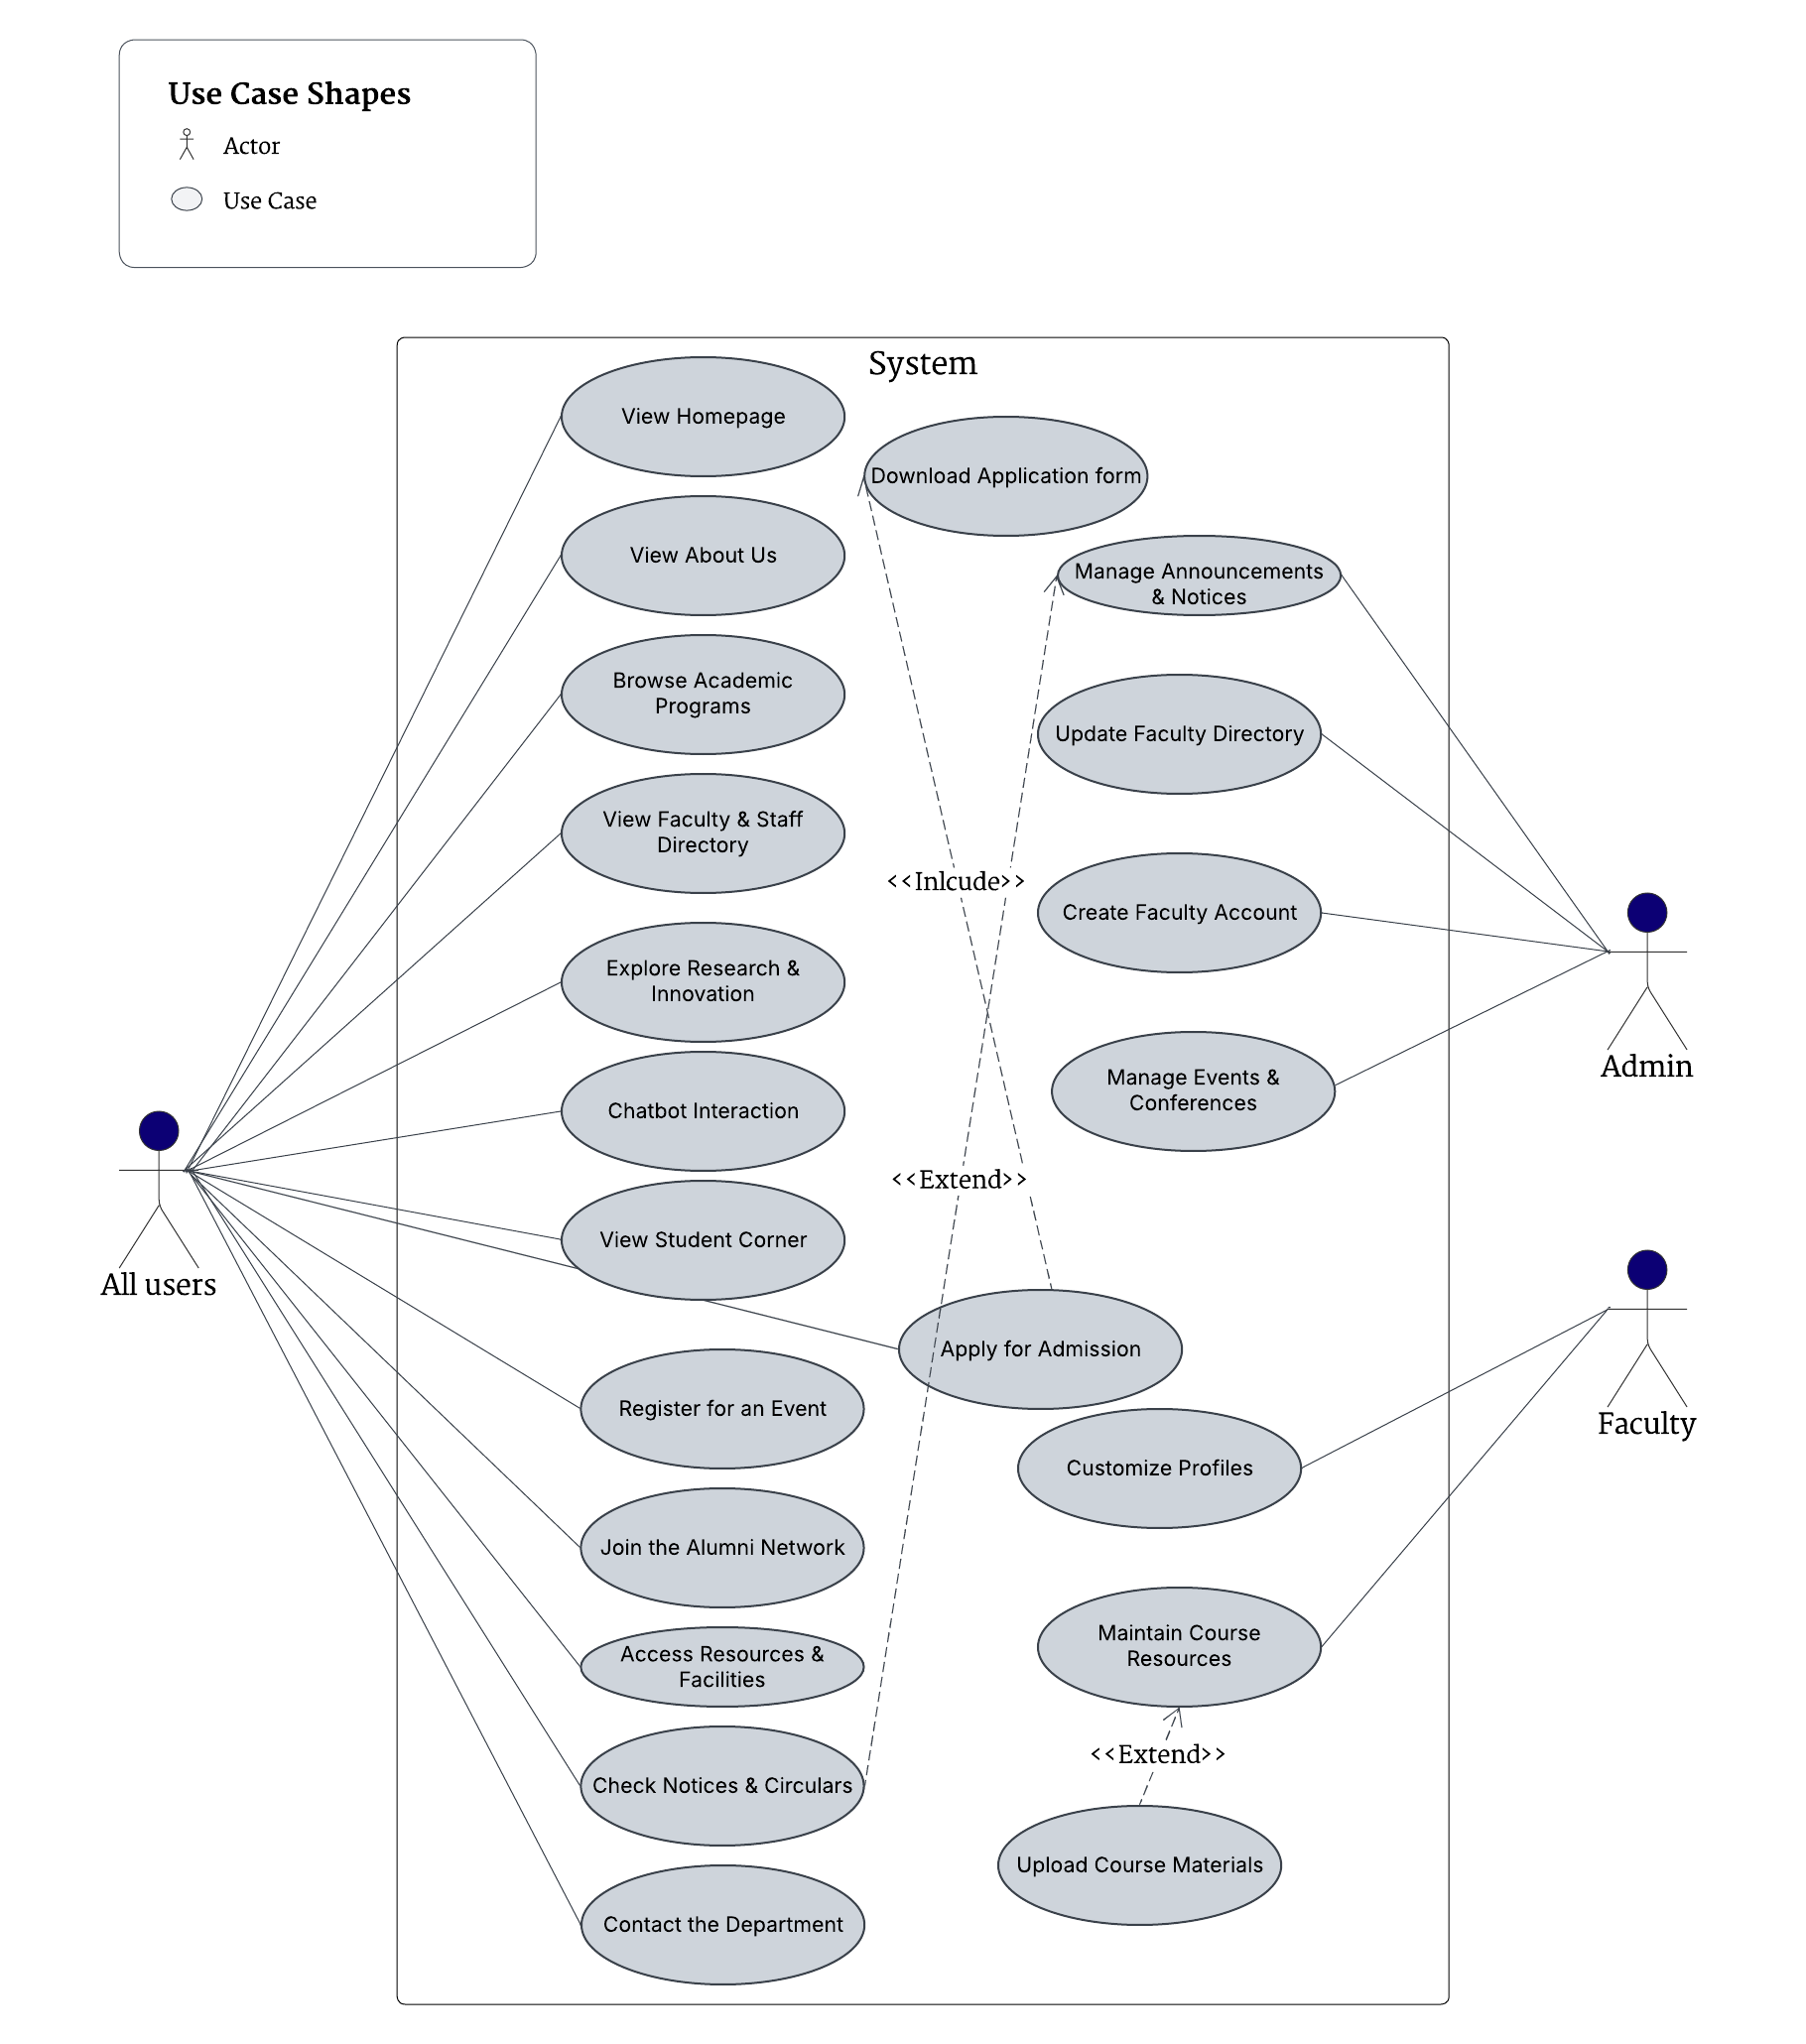
\includegraphics[width=\textwidth]{Usecase Diagram.png}
    \caption{Use case Diagram for TestCraft}
\end{figure}
\FloatBarrier
\newpage
\subsubsection{Dynamic Model}
\begin{customItemize}
    \item \textbf{Sequence Diagram}
    \FloatBarrier
    \begin{figure}[H]
        \centering
        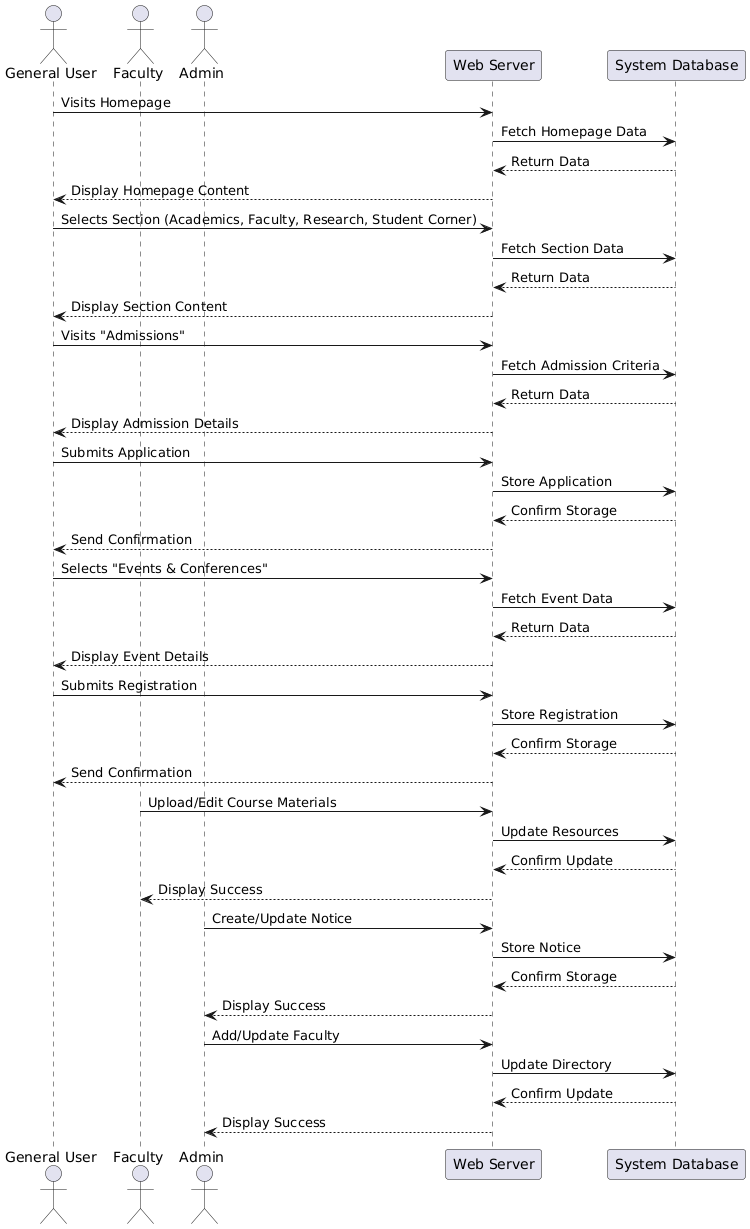
\includegraphics[height=16cm]{Seq Diagram.png}
        \caption{Sequence Diagram}
    \end{figure}
    \FloatBarrier
    \newpage
    \item \textbf{Activity Diagram}
    \FloatBarrier
    \begin{figure}[H]
        \centering
        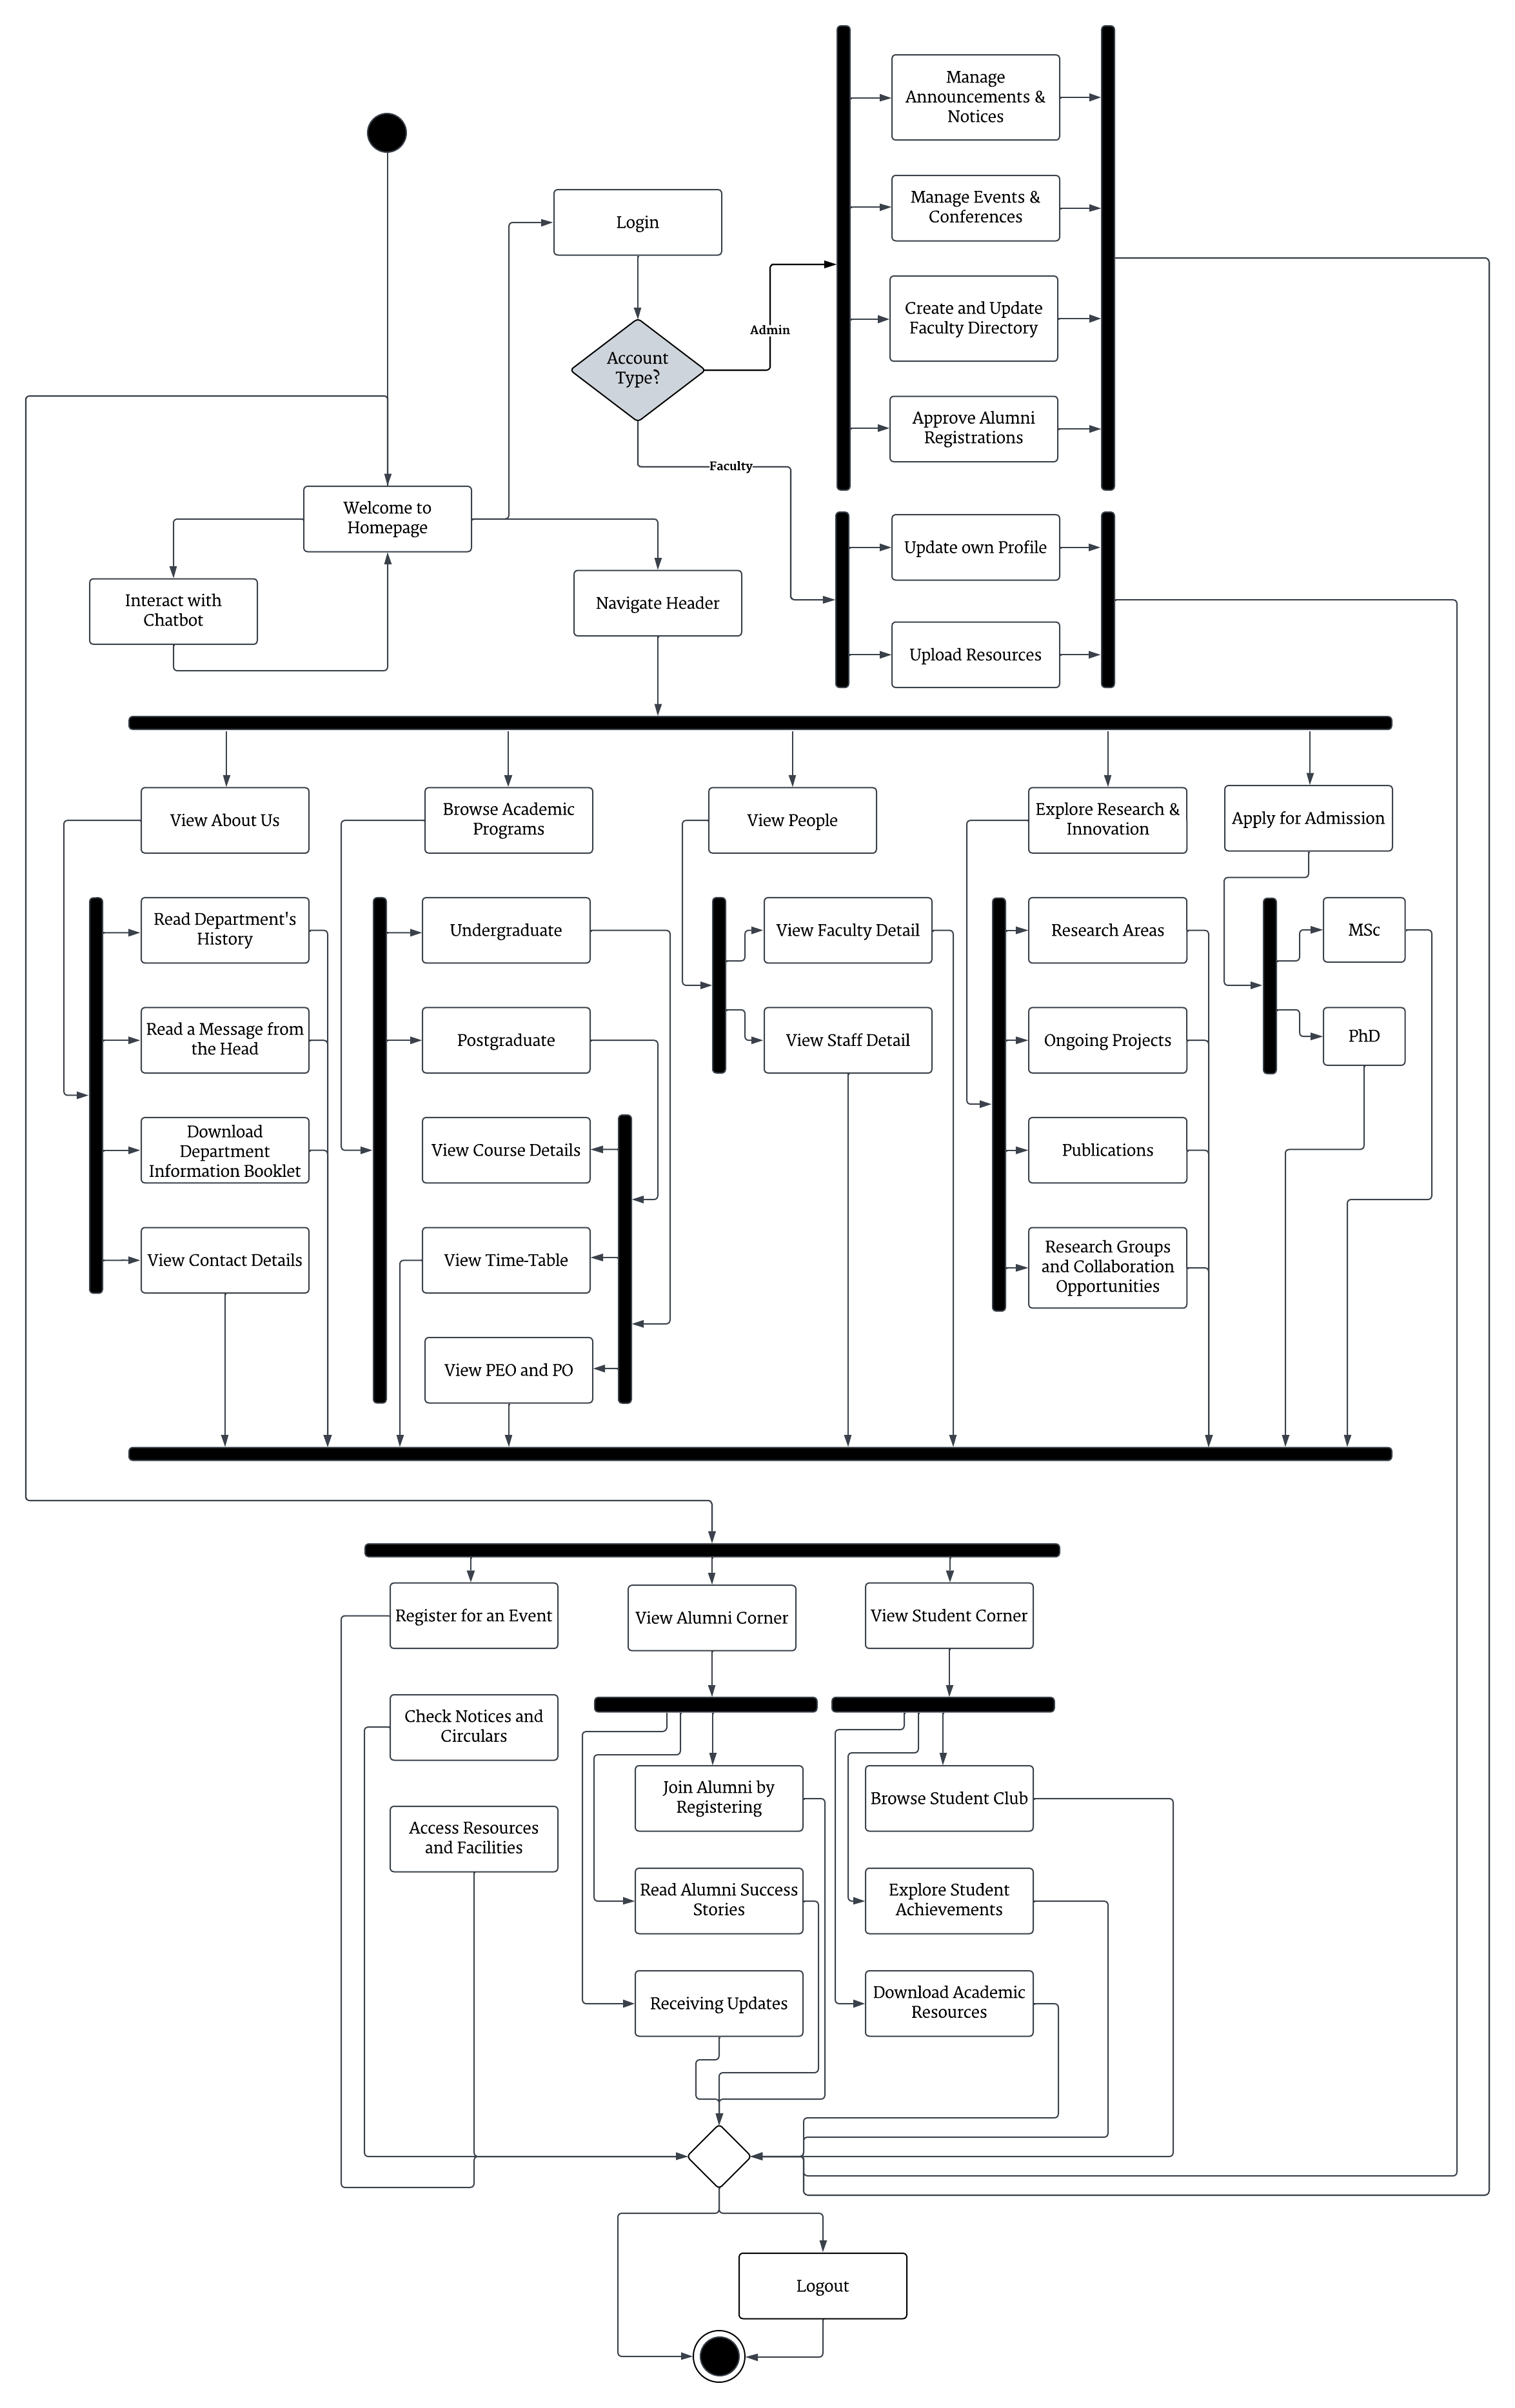
\includegraphics[height=17cm]{Activity Diagram.png}
        \caption{Activity Diagram}
    \end{figure}
    \FloatBarrier
    \newpage
    \item \textbf{State Diagrams}
    \FloatBarrier
    \begin{figure}[H]
        \centering
        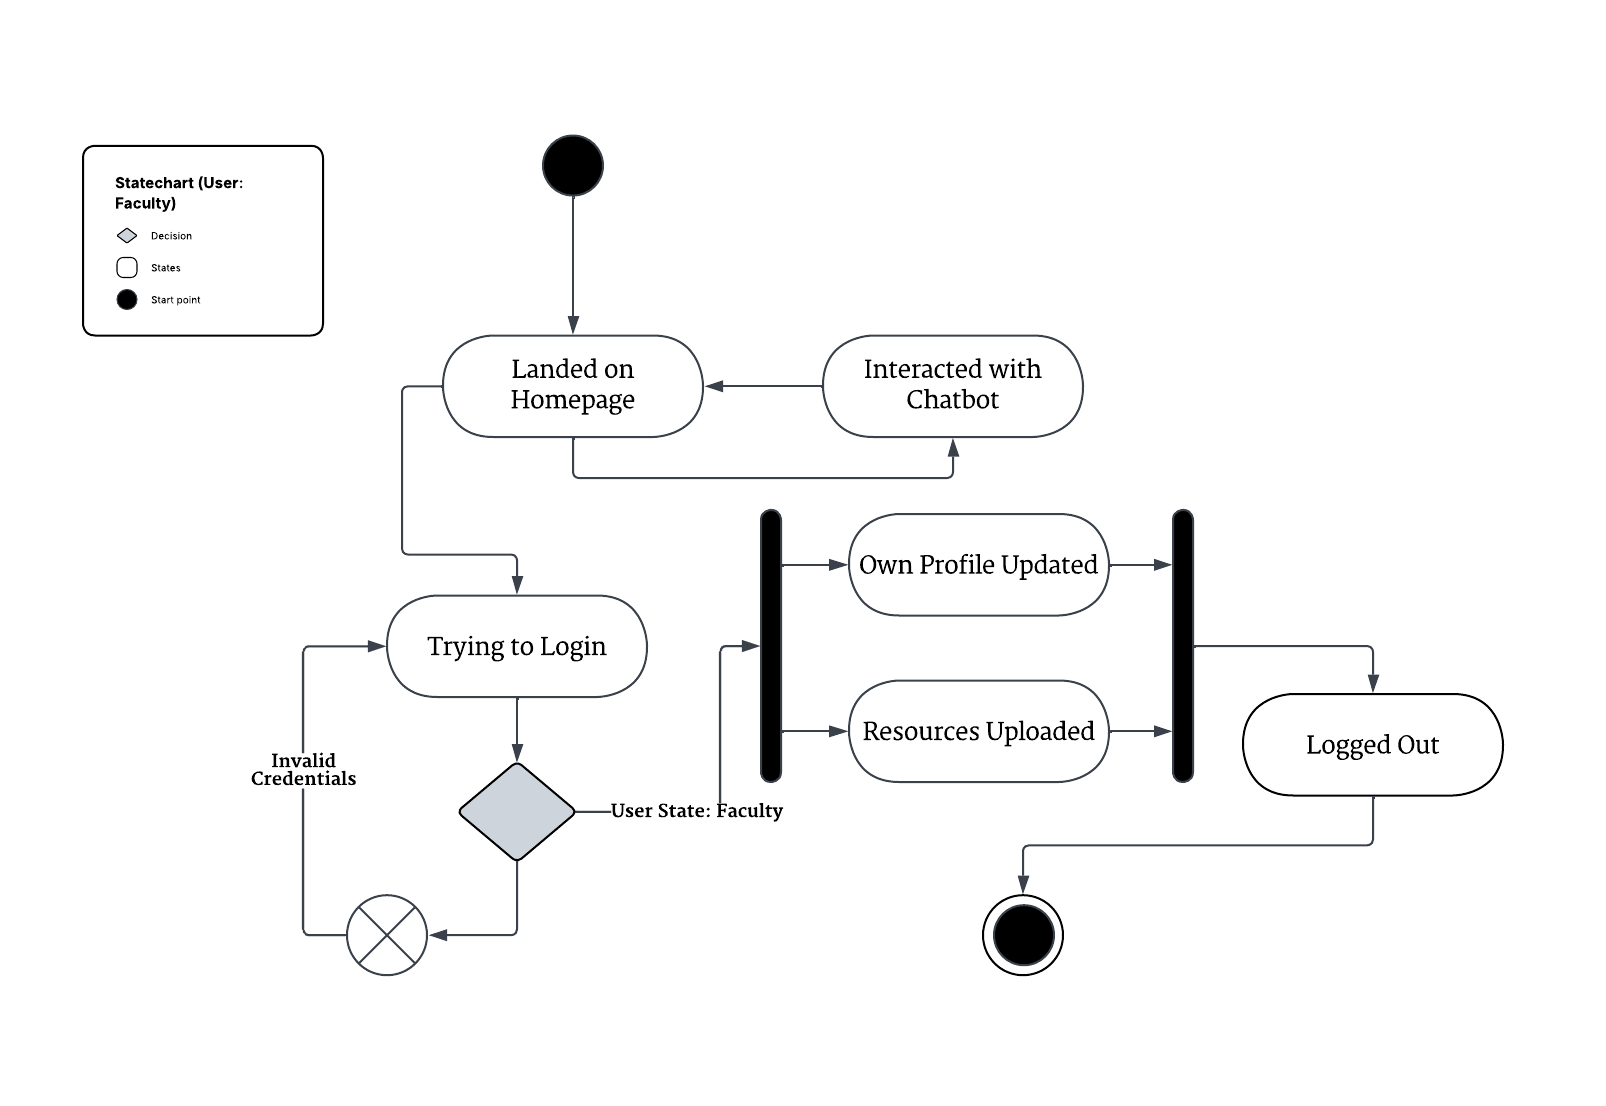
\includegraphics[height=6cm]{StateChart - Faculty.png}
        \caption{Faculty state diagram}
        \label{fig: Faculty state diagram}
    \end{figure}
    \FloatBarrier
    \FloatBarrier
    \begin{figure}[H]
        \centering
        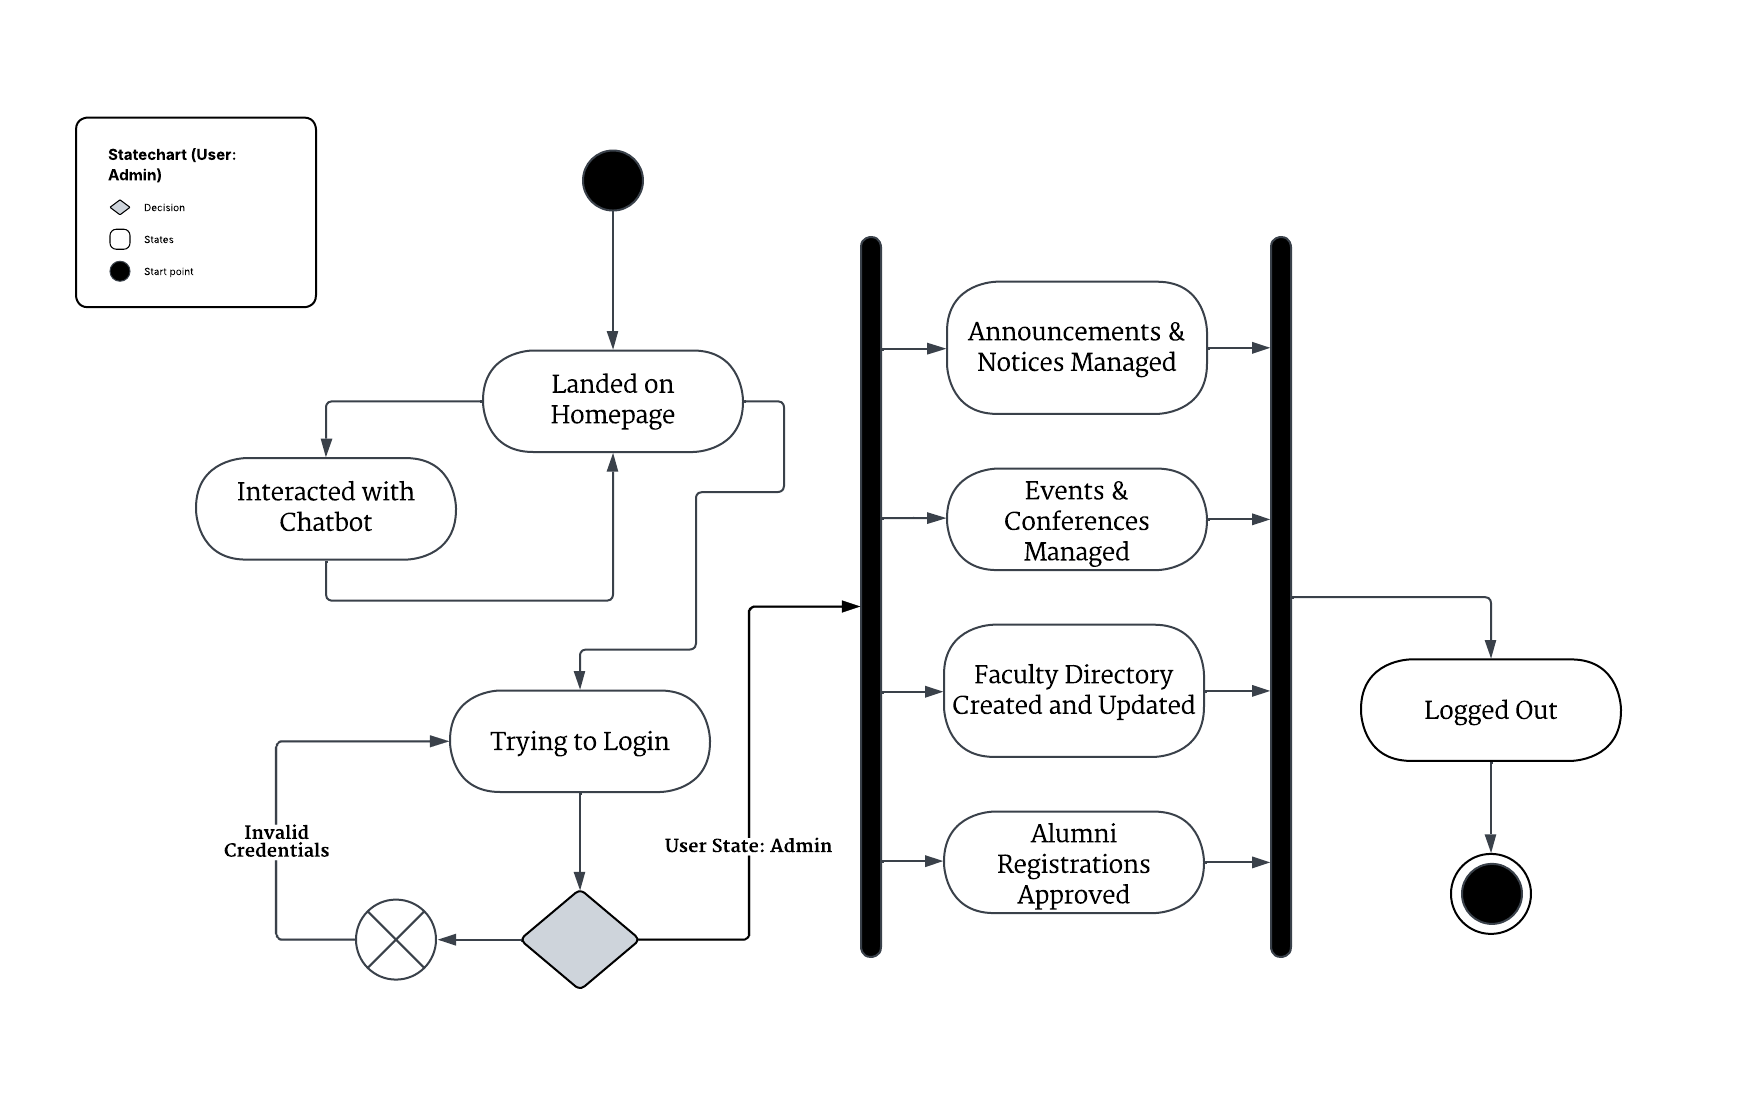
\includegraphics[height=8cm]{StateChart - Admin.png}
        \caption{Admin state diagram}
        \label{Admin state diagram}
    \end{figure}
    \FloatBarrier
    \FloatBarrier
    \begin{figure}[H]
        \centering
        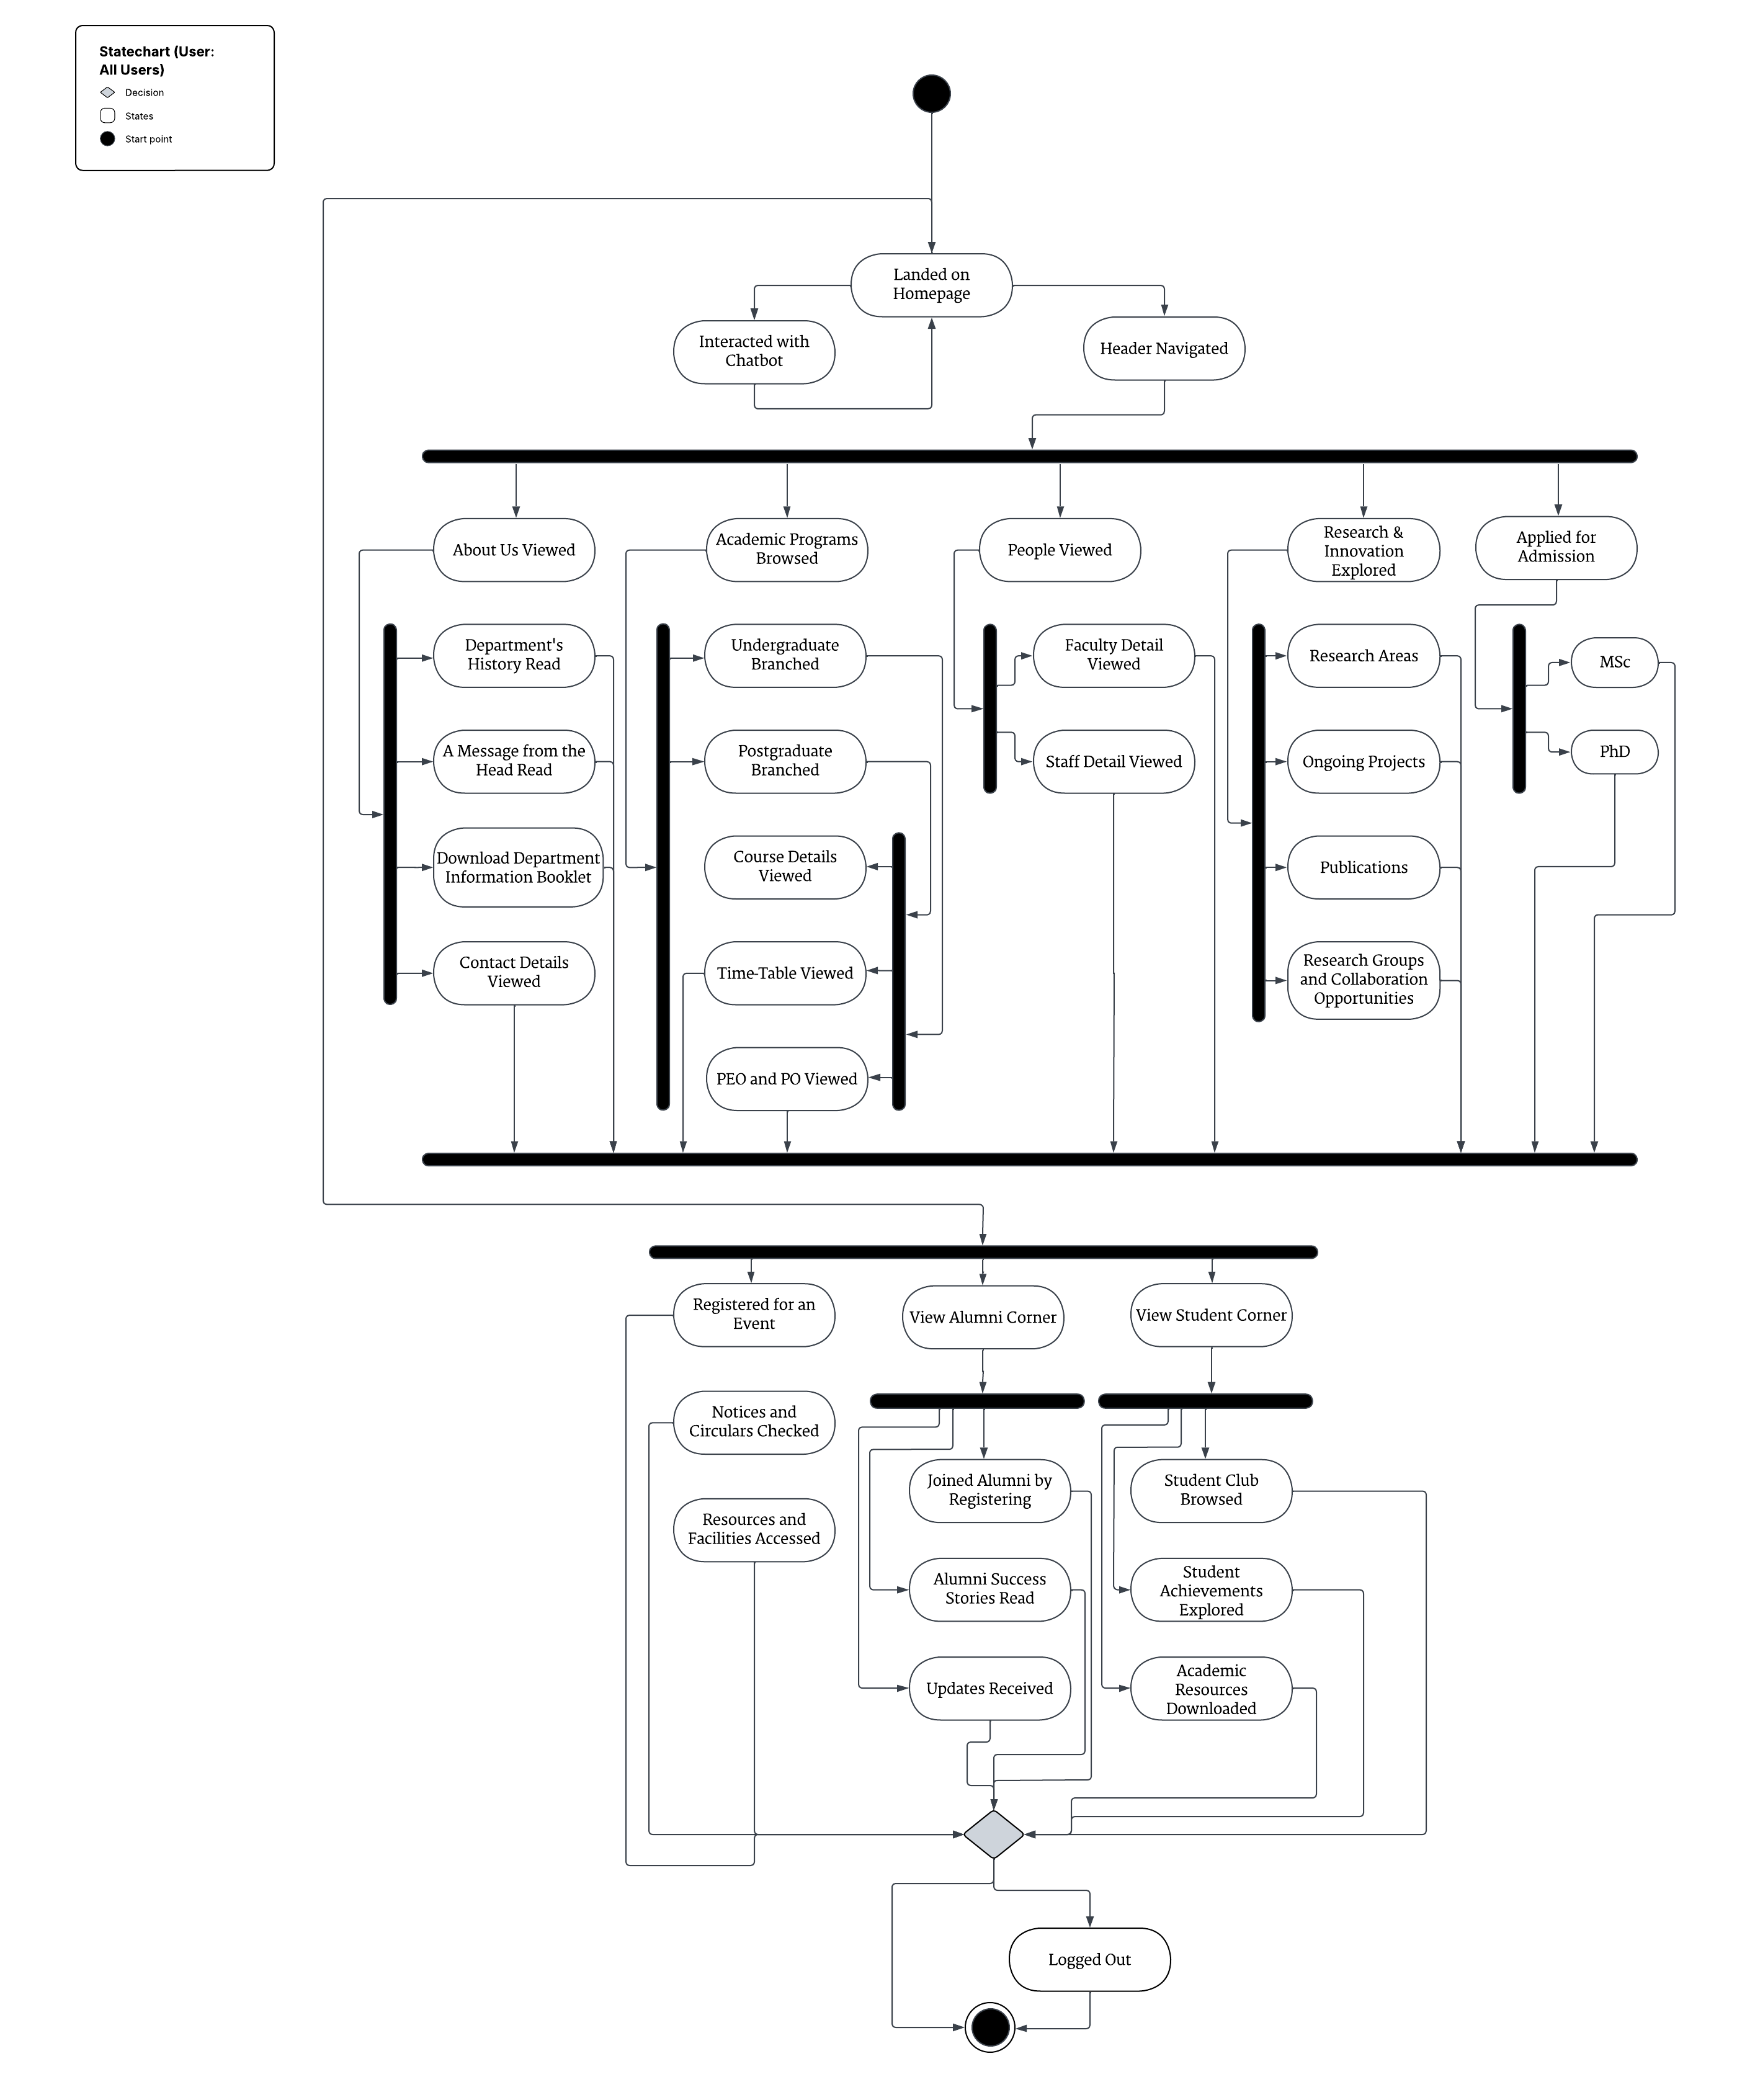
\includegraphics[height=17cm]{StateChart - All users.png}
        \caption{All users state diagram}
        \label{All users state diagram}
    \end{figure}
    \FloatBarrier
\end{customItemize}
\subsubsection{User Interface}
The prototype for this application was designed while maintaining a consistent color scheme and typography throughout the interface. The application is a web-based platform, and its responsiveness has been thoroughly tested across various devices, including desktops, laptops, iPads, and mobile phones. For development, we will use \ReactJS\space for the frontend, providing a dynamic and efficient user experience, while \FastAPI\space will be used for the backend, ensuring fast performance and scalability. The overall User Interface workflow is described below:

\begin{enumerate}
    \item \textbf{Homepage}
    \textbf{Workflow:}
    \begin{itemize}
        \item The user lands on the homepage.
        \item The homepage displays:
        \begin{itemize}
            \item Welcome message
            \item Department mission \& vision
            \item Announcements \& news
            \item Upcoming events
            \item Quick links (admissions, faculty, research, etc.)
        \end{itemize}
        \item Users can navigate to different sections from here.
    \end{itemize}

    \item \textbf{About Us}
    \textbf{Workflow:}
    \begin{itemize}
        \item User selects "About Us" from the navigation menu.
        \item Overview of the department is displayed.
        \item Users can read the message from the Head of the Department.
        \item History and achievements are accessible.
    \end{itemize}

    \item \textbf{Academics}
    \textbf{Workflow:}
    \begin{itemize}
        \item User selects "Academics."
        \item A list of academic programs is displayed, including:
        \begin{itemize}
            \item Undergraduate Programs (course structure, syllabus, credit details)
            \item Postgraduate Programs
            \item PhD Programs
        \end{itemize}
        \item Users can access:
        \begin{itemize}
            \item Course Catalog
            \item Class schedules \& timetables
            \item Academic Calendar
        \end{itemize}
    \end{itemize}

    \item \textbf{Faculty \& Staff}
    \textbf{Workflow:}
    \begin{itemize}
        \item User selects "Faculty \& Staff."
        \item Faculty directory displays names, designations, specializations, contact details, and research backgrounds.
        \item Users can access faculty members' LinkedIn and Google Scholar profiles.
        \item Staff details and office hours are available.
    \end{itemize}

    \item \textbf{Research \& Innovation}
    \textbf{Workflow:}
    \begin{itemize}
        \item User selects "Research \& Innovation."
        \item Research areas are displayed with detailed descriptions.
        \item Publications are available for browsing or download.
        \item Research groups, labs, and ongoing projects are listed.
        \item Collaboration opportunities and research funding information are accessible.
    \end{itemize}

    \item \textbf{Admissions}
    \textbf{Workflow:}
    \begin{itemize}
        \item User selects "Admissions."
        \item Admission criteria and process for MSc and PhD programs are outlined.
        \item Application forms are available for download.
        \item Scholarship and financial aid details are provided.
        \item Users can browse FAQs for common queries.
    \end{itemize}

    \item \textbf{Student Corner}
    \textbf{Workflow:}
    \begin{itemize}
        \item User selects "Student Corner."
        \item Student clubs and organizations are listed with descriptions and join options.
        \item Student achievements are showcased.
        \item Academic resources, including lecture notes and previous question papers, are accessible.
    \end{itemize}

    \item \textbf{Events \& Conferences}
    \textbf{Workflow:}
    \begin{itemize}
        \item User selects "Events \& Conferences."
        \item Upcoming workshops, seminars, hackathons, and coding competitions are displayed.
        \item Users can register for events directly from this section.
        \item Past event highlights include images and videos.
    \end{itemize}

    \item \textbf{Alumni}
    \textbf{Workflow:}
    \begin{itemize}
        \item User selects "Alumni."
        \item Success stories are displayed.
        \item Alumni network and event details are accessible.
    \end{itemize}

    \item \textbf{Resources \& Facilities}
    \textbf{Workflow:}
    \begin{itemize}
        \item User selects "Resources \& Facilities."
        \item Information about laboratories, equipment, and computing facilities is available.
        \item Library and digital resources are listed.
        \item Department policies can be viewed or downloaded.
    \end{itemize}

    \item \textbf{Notices \& Circulars}
    \textbf{Workflow:}
    \begin{itemize}
        \item User selects "Notices \& Circulars."
        \item Official announcements and examination notices are displayed.
        \item Departmental policies and updates are listed.
    \end{itemize}

    \item \textbf{Contact Us}
    \textbf{Workflow:}
    \begin{itemize}
        \item User selects "Contact Us."
        \item Department location and an interactive map are displayed.
        \item Email and phone contact details are provided.
        \item An inquiry form allows users to submit questions directly.
    \end{itemize}
\end{enumerate}

\subsubsection{Software Interface}
\paragraph{Front-End (Presentation Layer)}
\begin{itemize}
    \item \textbf{Web Framework (\ReactJS)}: Handles the UI with reusable components and client-side rendering.
    \item \textbf{Styling (\CSS)}: Styles the user interface, including layout, fonts, and colors.
    \item \textbf{Programming Language (\JavaScript)}: Enhances interactivity and dynamic behavior of the web application.
\end{itemize}

\paragraph{Back-End (Logic Layer)}
\begin{itemize}
    \item \textbf{Programming Language (\Python)}: Manages server-side logic, API requests, and data processing.
    \item \textbf{Web Framework (\FastAPI)}: Provides a fast and efficient backend with API routing, authentication, and database interactions.
    \item \textbf{Database (\PostgreSQL/\textbf{\textit{MongoDB}} )}: Stores all application data, including user information, department details, research data, event details, and notices.
\end{itemize}

\paragraph{Data Flow}
\begin{itemize}
    \item \textbf{Incoming Data:}
    \begin{itemize}
        \item \textbf{User Input}: Users provide data through web forms in the React frontend, such as sign-up details, event registrations, and feedback.
        \item \textbf{API Requests (Optional)}: If integrating with external \textit{API}s (e.g., research publications, funding details, or alumni networks), \textit{FastAPI} will handle incoming data from these sources.
    \end{itemize}
    \item \textbf{Outgoing Data:}
    \begin{itemize}
        \item \textbf{API Responses}: \textit{FastAPI} sends structured \textit{JSON} responses to the React frontend, which dynamically updates the UI.
        \item \textbf{Database Interactions}: \textit{FastAPI} communicates with \textit{PostgreSQL/MongoDB} to store and retrieve data, such as faculty details, academic records, research projects, and student information.
        \item \textbf{Emails}: The backend can send automated emails for password change requests
        \item \textbf{API Interactions (Optional)}: If needed, \textit{FastAPI} can send data to external services for research data integration, collaboration tools, or alumni networking.
    \end{itemize}
\end{itemize}

\paragraph{Communication Services}
\begin{itemize}
    \item \textbf{Database Management System (\PostgreSQL\space or \textit{MongoDB})}: The chosen database management system provides functionalities for storing, retrieving, and manipulating data within the database.
\end{itemize}

\paragraph{Implementation Constraints}
\begin{itemize}
    \item \textbf{Data Security}: Sensitive user data (passwords, personal information) should be stored securely using hashing algorithms. Research and academic records must be protected from unauthorized access.
    \item \textbf{API Authentication}: If external APIs are used, proper authentication methods will be established to securely exchange data.
    \item \textbf{Role-Based Access Control}: Faculty, students, and administrators should have different access permissions to manage data effectively.
\end{itemize}

\subsubsection{Hardware Interface}
As per the plan for this project, the hardware parts include the servers for hosting the app and the devices clients use to access it online. The way the software connects with the hardware involves supporting different web browsers like Chrome, Firefox, and Safari, and making sure the devices have internet access to reach the app. The physical aspects of this connection include the network linking client devices and servers, the specifications of server hardware, and how much data the server can store. To communicate between client devices and servers, the system will use HTTP over the internet, with SSL encryption for safety. The hardware needs to meet certain requirements to run the app, outlined in the installation and deployment guides. However, since this is a web app, it can work on any device with an internet connection.



\section{Supporting Information}
\begin{customItemize}
    \item \textbf{Installation}
    \begin{itemize}
        \item \textbf{Frontend:}  
        If \NodeJS\space is already installed, run the following commands in the terminal to set up and start the \ReactJS\space frontend:  
        \begin{verbatim}
        npm install
        npm run start
        \end{verbatim}

        \item \textbf{Backend:}  
        If \Python\space is already installed, run the following commands in the terminal to set up and start the \FastAPI\space backend:  
        \begin{verbatim}
        pip install -r requirements.txt
        uvicorn main:app --reload
        \end{verbatim}
    \end{itemize}

    \item \textbf{Deployment} \newline
    \begin{itemize}
        \item \textbf{Method 1:} Deploy frontend server into \textbf{\textit{Vercel}} from the git repository pretty easily. See \url{https://vercel.com/} for more information
        
            And then deploy backend server into any cloud service (\textit{\textbf{Google Cloud, AWS}} etc)
        
        \item \textbf{Method 2:} Containerize the application using \textbf{\textit{Docker}} and host it from a \textbf{\textit{Linux}} based cloud server. Or manually set up a custom \textbf{\textit{Linux}} server and host under the domain \textbf{\textit{du.ac.bd}}
    \end{itemize}
\end{customItemize}
\end{document}
